\chapter{RESULTS AND DISCUSSION}
\label{ch:results}

\section{RESULTS}
This section presents the empirical findings obtained by executing the complete machine learning and customer segmentation pipeline on the benchmark IBM Telco dataset. All evaluations were conducted on the isolated, held-out test partition ($N=\datasetTestCount{}$ records, comprising 1,035 retained customers and 374 churned customers), ensuring that reported performance reflects authentic operational generalization.

\subsection{Supervised Classification Model Comparison}
The performance of the four primary classification algorithms across all standard evaluation metrics is summarized in Table~\ref{tab:model_comparison}.

\begin{table}[H]
\centering
\caption{Model Performance on the Held-Out Test Set ($N=1,409$)}
\label{tab:model_comparison}
\begin{tabular}{lcccccc}
\toprule
\textbf{Model} & \textbf{Accuracy} & \textbf{Precision} & \textbf{Recall} & \textbf{F1-Score} & \textbf{ROC-AUC} & \textbf{PR-AUC} \\
\midrule
Random Forest & 0.7559 & 0.5276 & 0.7674 & 0.6253 & 0.8427 & 0.6554 \\
Support Vector Machine & 0.7452 & 0.5133 & 0.7727 & 0.6169 & 0.8213 & 0.5861 \\
Logistic Regression & 0.7381 & 0.5043 & 0.7834 & 0.6136 & 0.8415 & 0.6325 \\
Multi-Layer Perceptron & 0.8034 & 0.6678 & 0.5160 & 0.5822 & 0.8342 & 0.6225 \\
\bottomrule
\end{tabular}
\end{table}

As documented in Table~\ref{tab:model_comparison}, \textbf{\bestModelName{}} achieved the highest overall balance across the competitive metric suite, attaining an F1-score of \textbf{\bestModelFOne{}}, a Receiver Operating Characteristic Area Under the Curve (ROC-AUC) of \textbf{\bestModelRocAuc{}}, and a Precision-Recall Area Under the Curve (PR-AUC) of \textbf{\bestModelPrAuc{}}. Support Vector Machine and Logistic Regression demonstrated closely matched performance, achieving F1-scores of \SupportVectorMachineFOne{} and \LogisticRegressionFOne{}, respectively. Logistic Regression attained the highest raw churn sensitivity (Recall = \LogisticRegressionRec{}), successfully detecting 293 of the 374 actual churners in the test split. Conversely, the Multi-Layer Perceptron favored precision over recall, achieving the highest overall accuracy (80.34\%) and precision (66.78\%), but registering a lower recall of 51.60\%.

Figure~\ref{fig:model_comparison_bar} visualizes the multi-metric comparison across the four algorithms.

\begin{figure}[H]
    \centering
    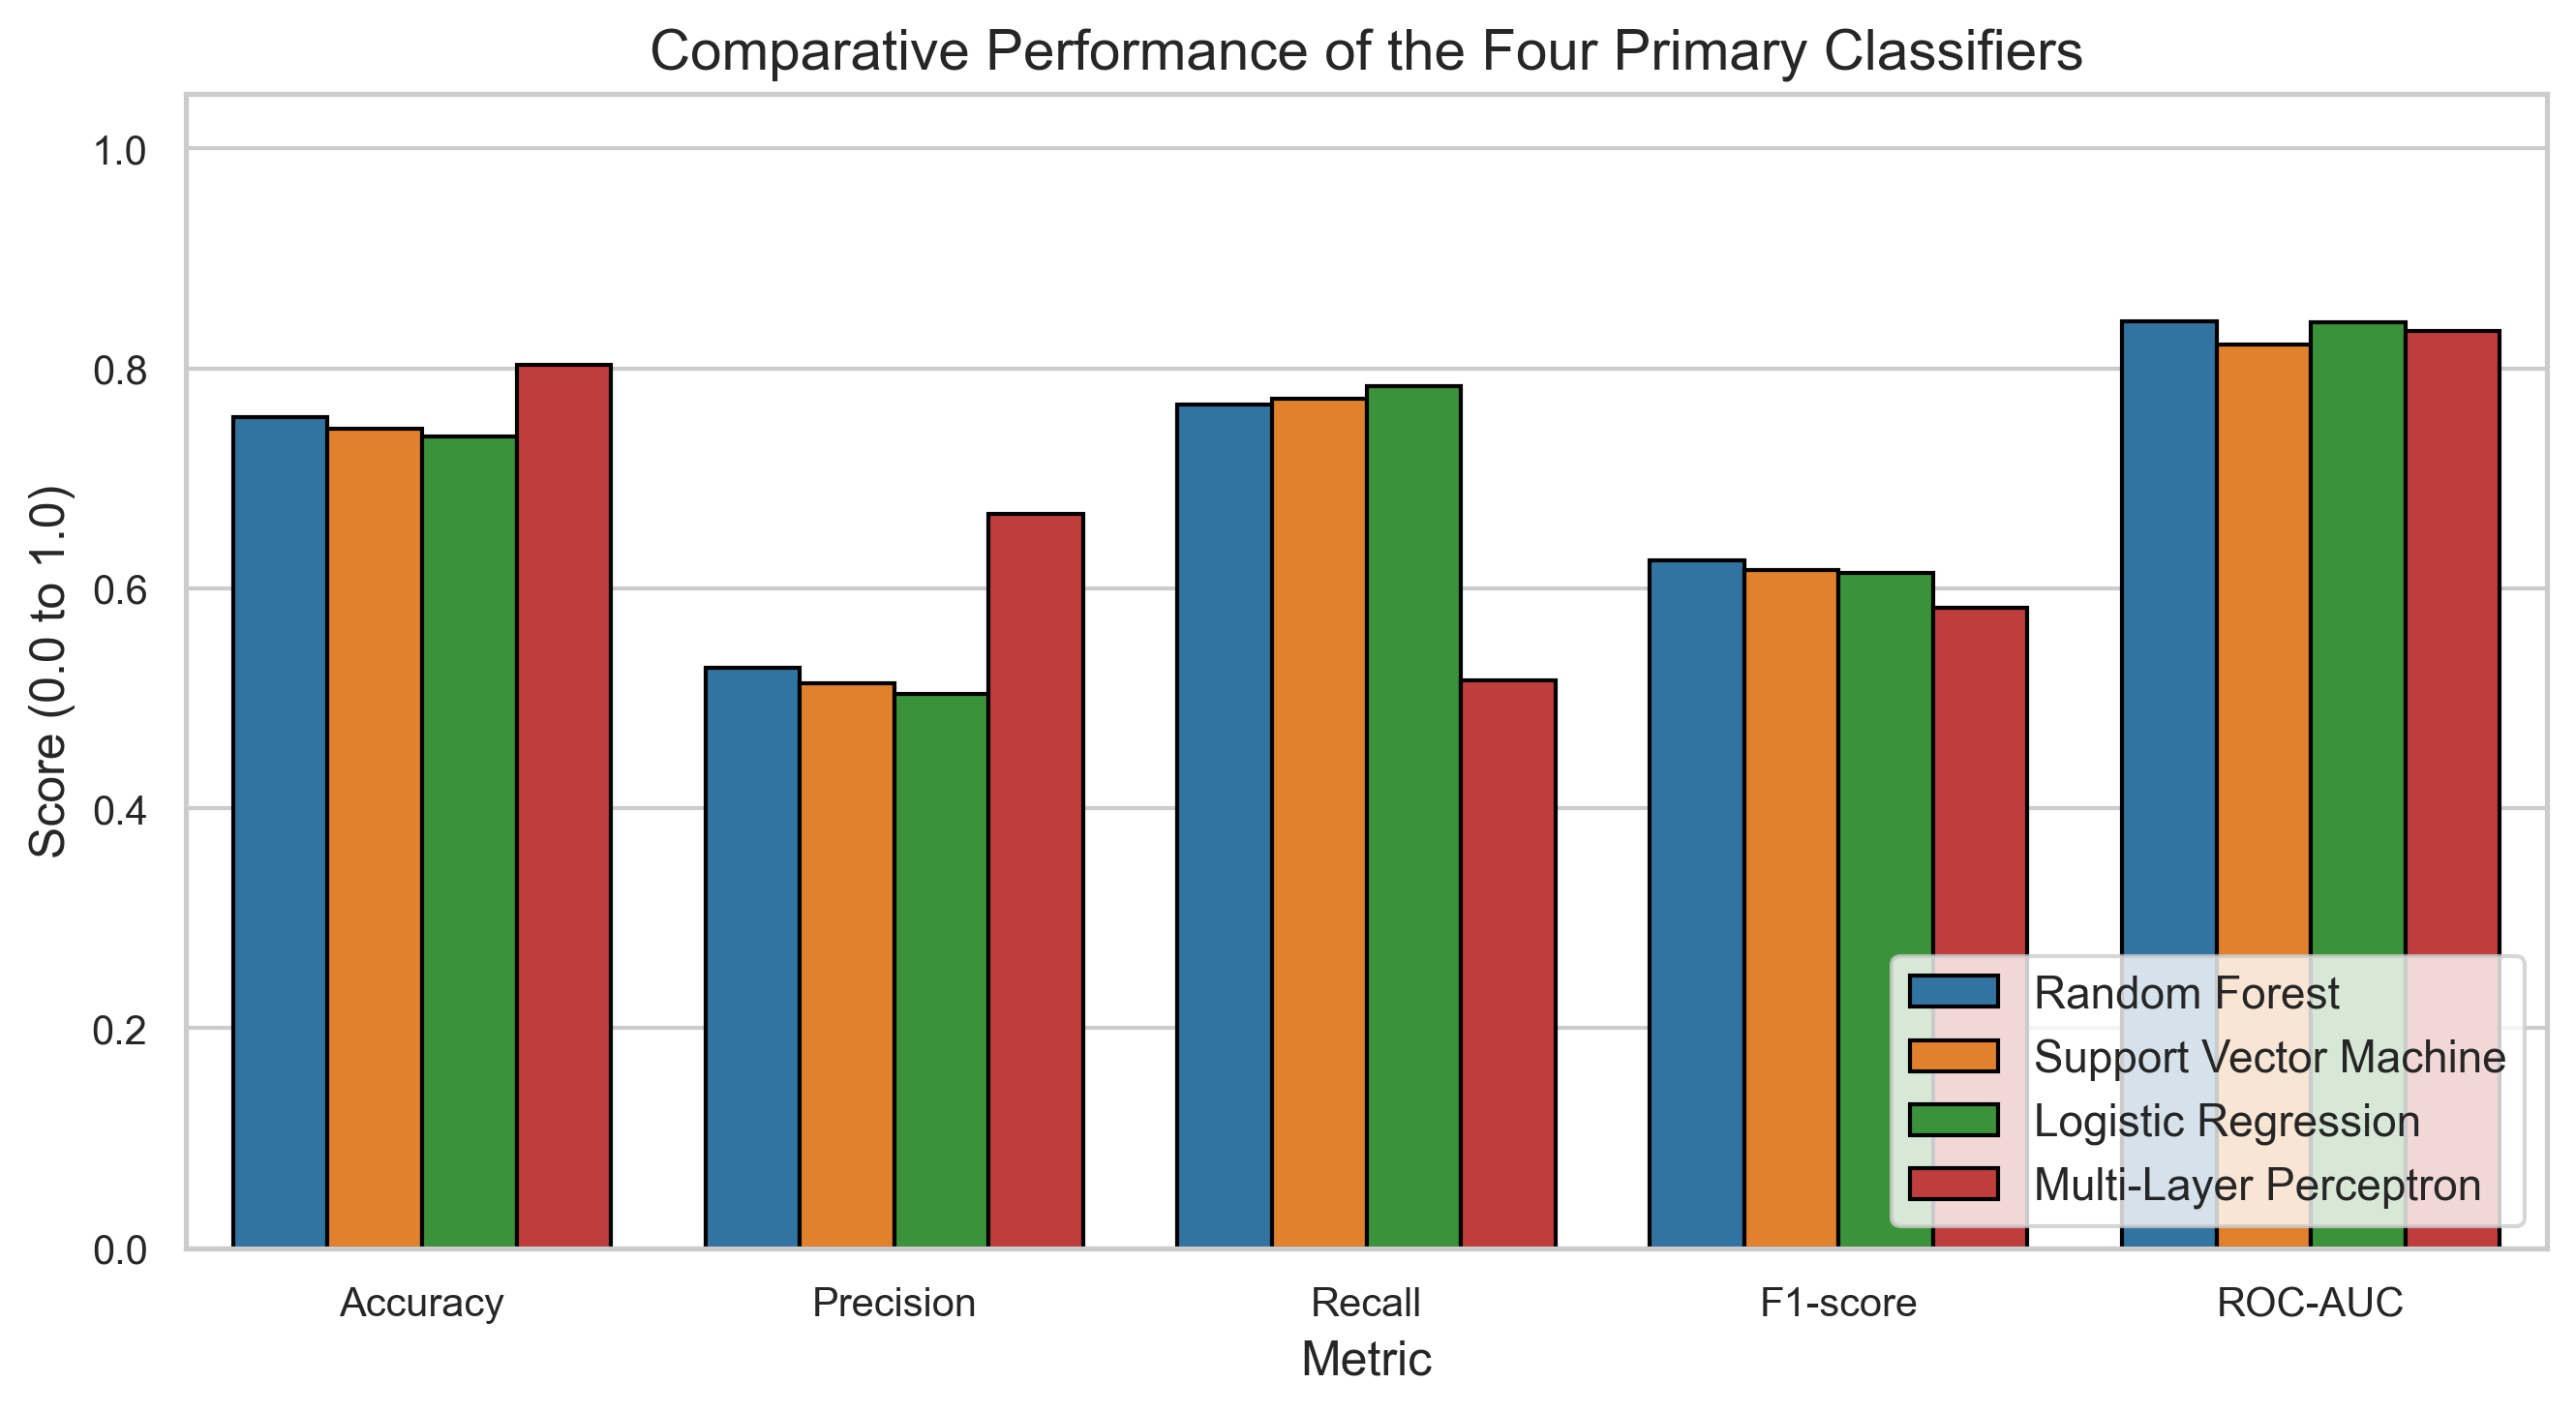
\includegraphics[width=0.88\textwidth]{figures/eval_model_comparison_bar.png}
    \caption{Comparative Metric Evaluation Across the Four Primary Classifiers}
    \label{fig:model_comparison_bar}
\end{figure}

\subsection{Confusion Matrices and Error Breakdown}
To evaluate operational classification errors, Figure~\ref{fig:confusion_matrices} displays the empirical confusion matrices for all four classifiers on the 1,409 test records.

\begin{figure}[H]
    \centering
    \begin{subfigure}[b]{0.48\textwidth}
        \centering
        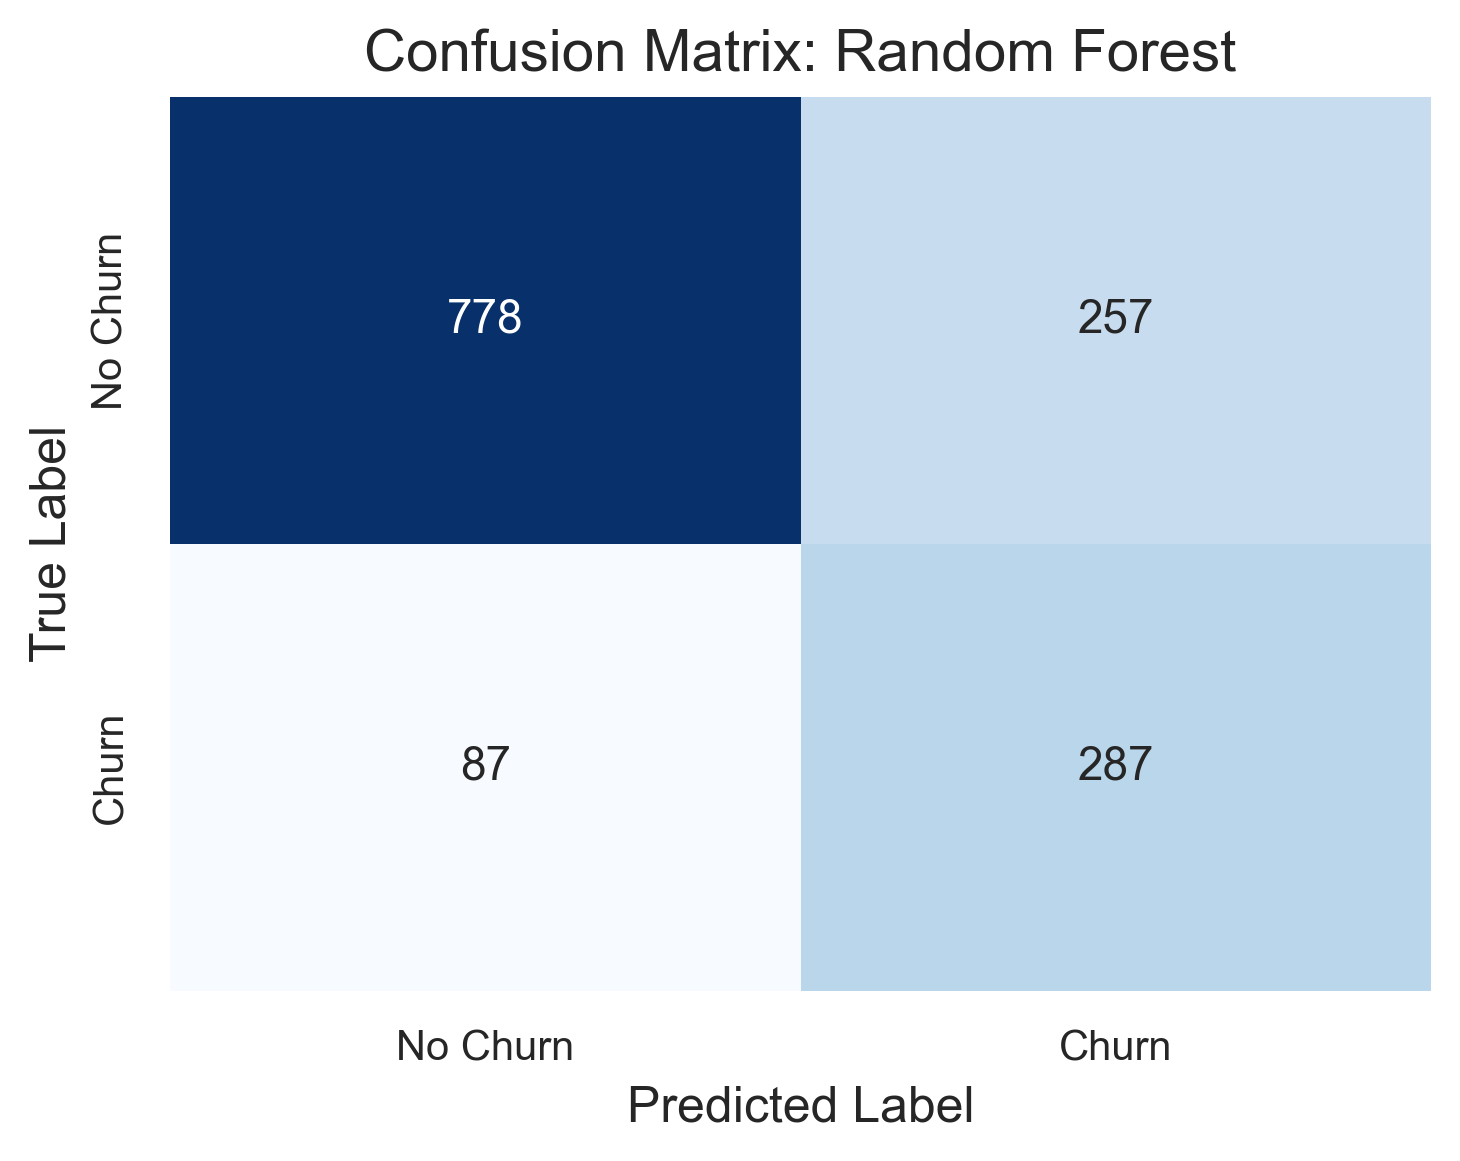
\includegraphics[width=\textwidth]{figures/confusion_matrix_random_forest.png}
        \caption{Random Forest Classifier}
        \label{fig:cm_rf}
    \end{subfigure}
    \hfill
    \begin{subfigure}[b]{0.48\textwidth}
        \centering
        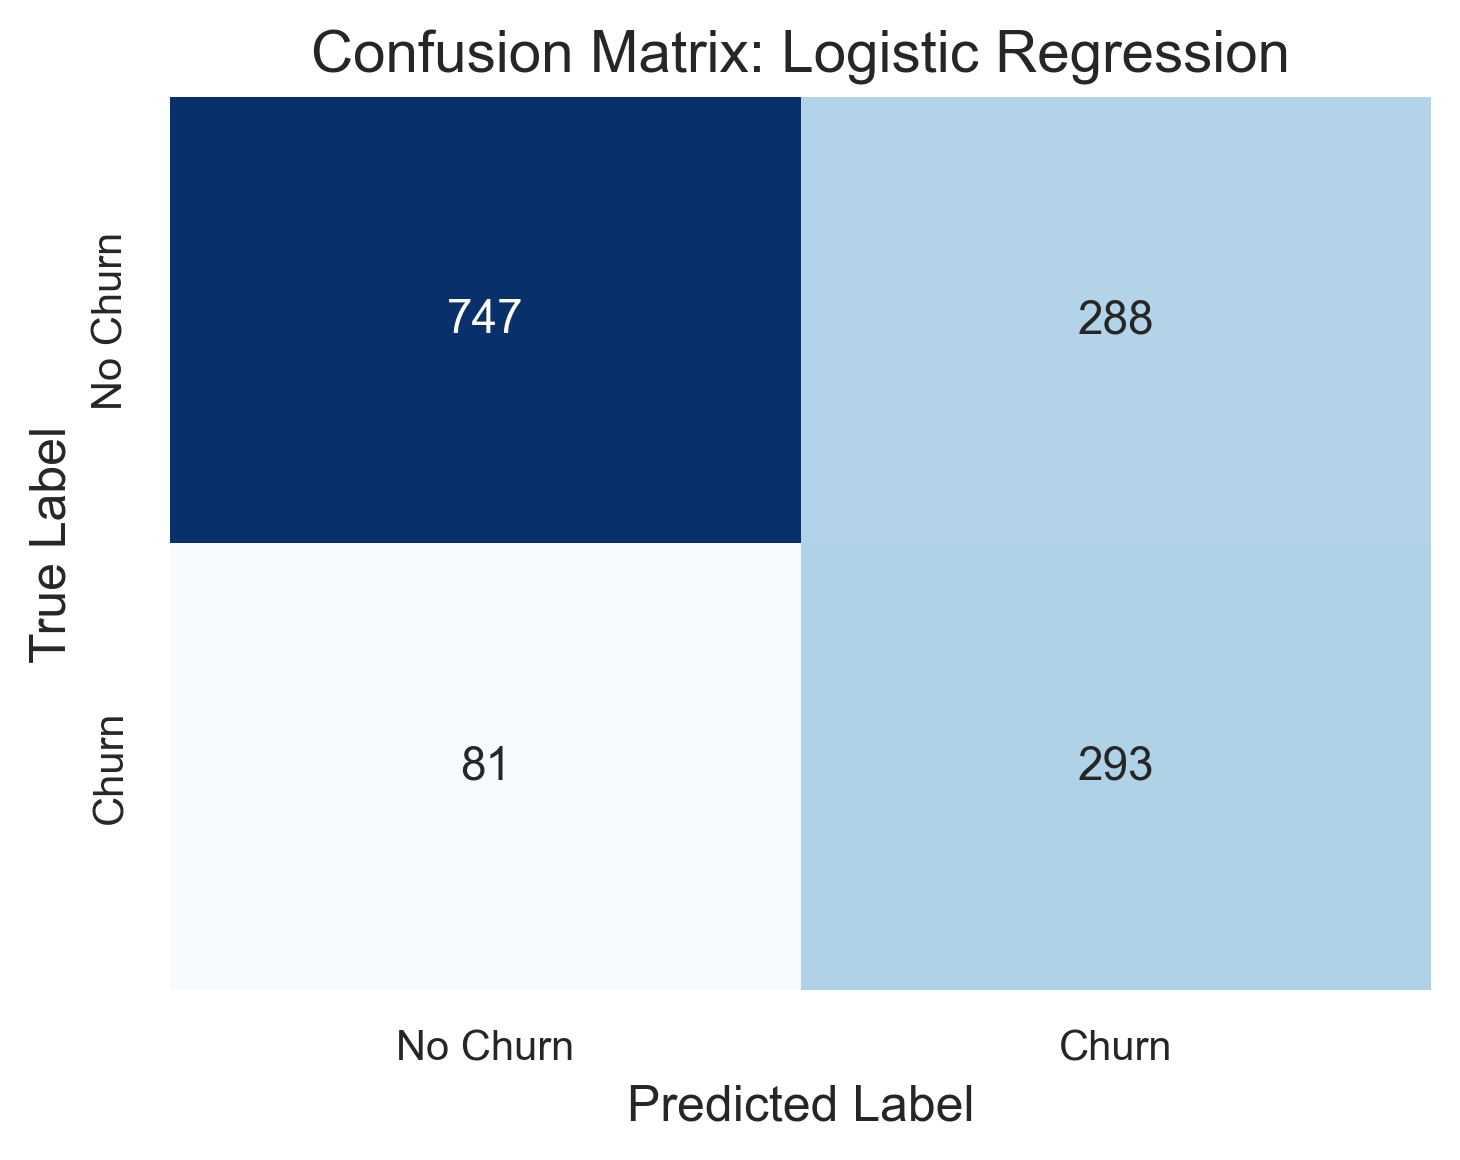
\includegraphics[width=\textwidth]{figures/confusion_matrix_logistic_regression.png}
        \caption{Logistic Regression Baseline}
        \label{fig:cm_lr}
    \end{subfigure}
    \\[0.3cm]
    \begin{subfigure}[b]{0.48\textwidth}
        \centering
        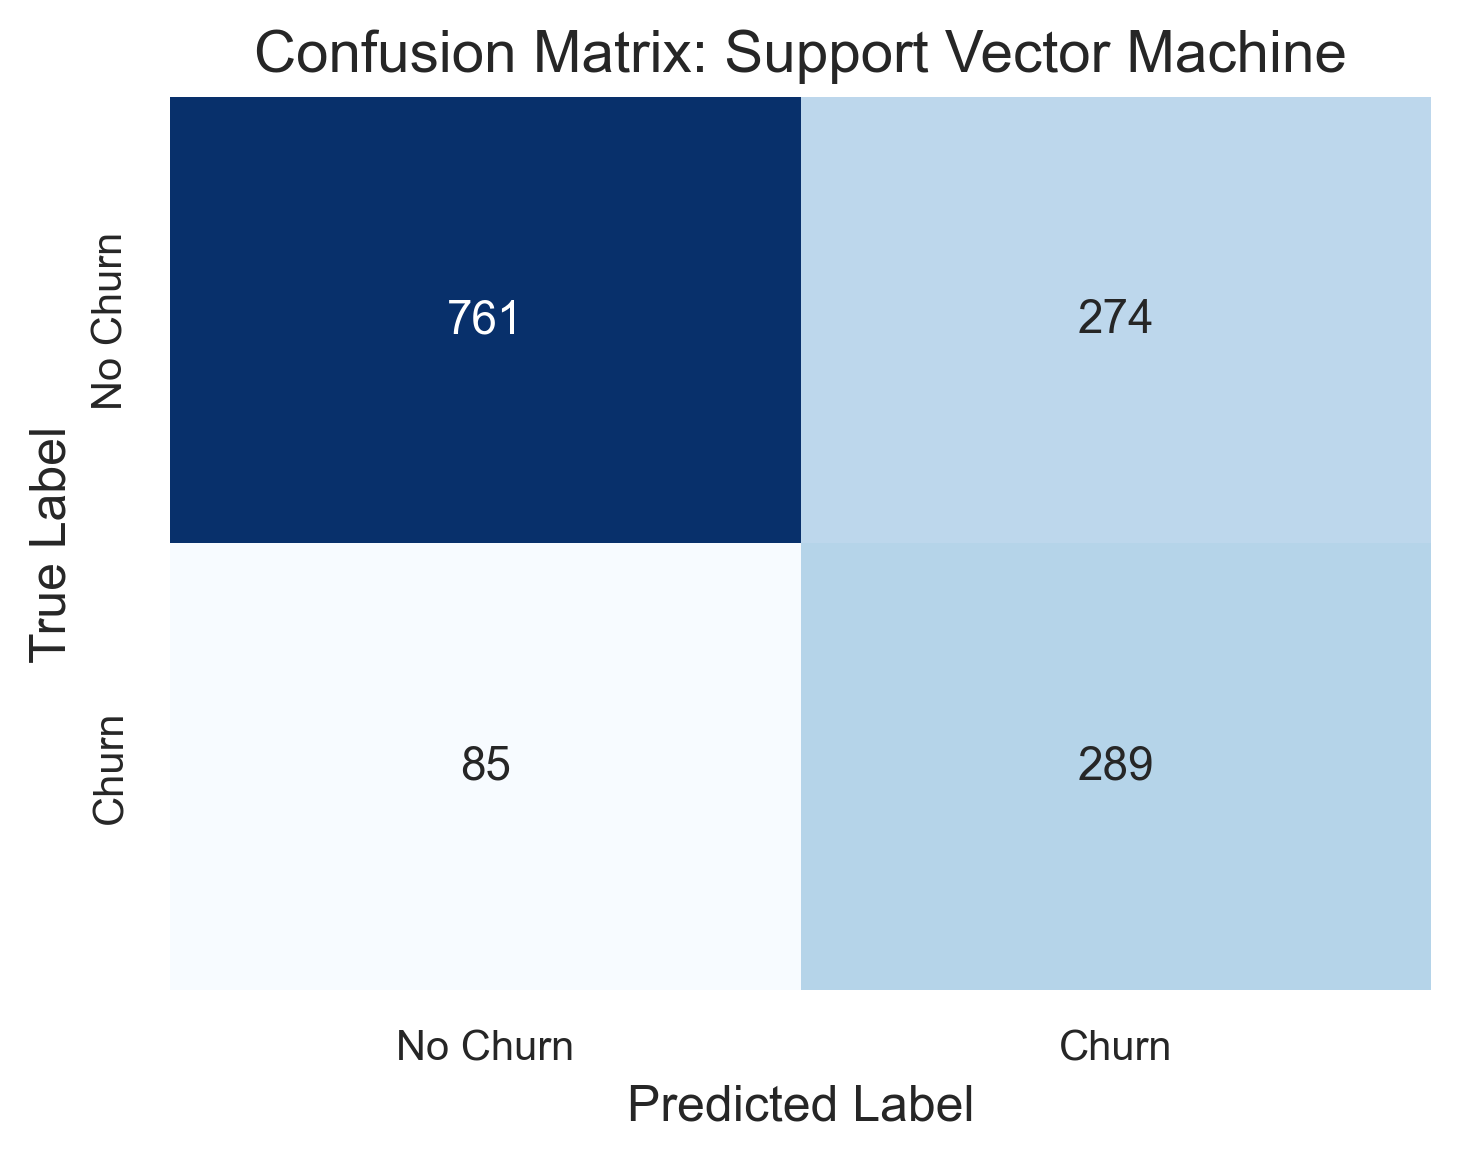
\includegraphics[width=\textwidth]{figures/confusion_matrix_support_vector_machine.png}
        \caption{Support Vector Machine (RBF)}
        \label{fig:cm_svm}
    \end{subfigure}
    \hfill
    \begin{subfigure}[b]{0.48\textwidth}
        \centering
        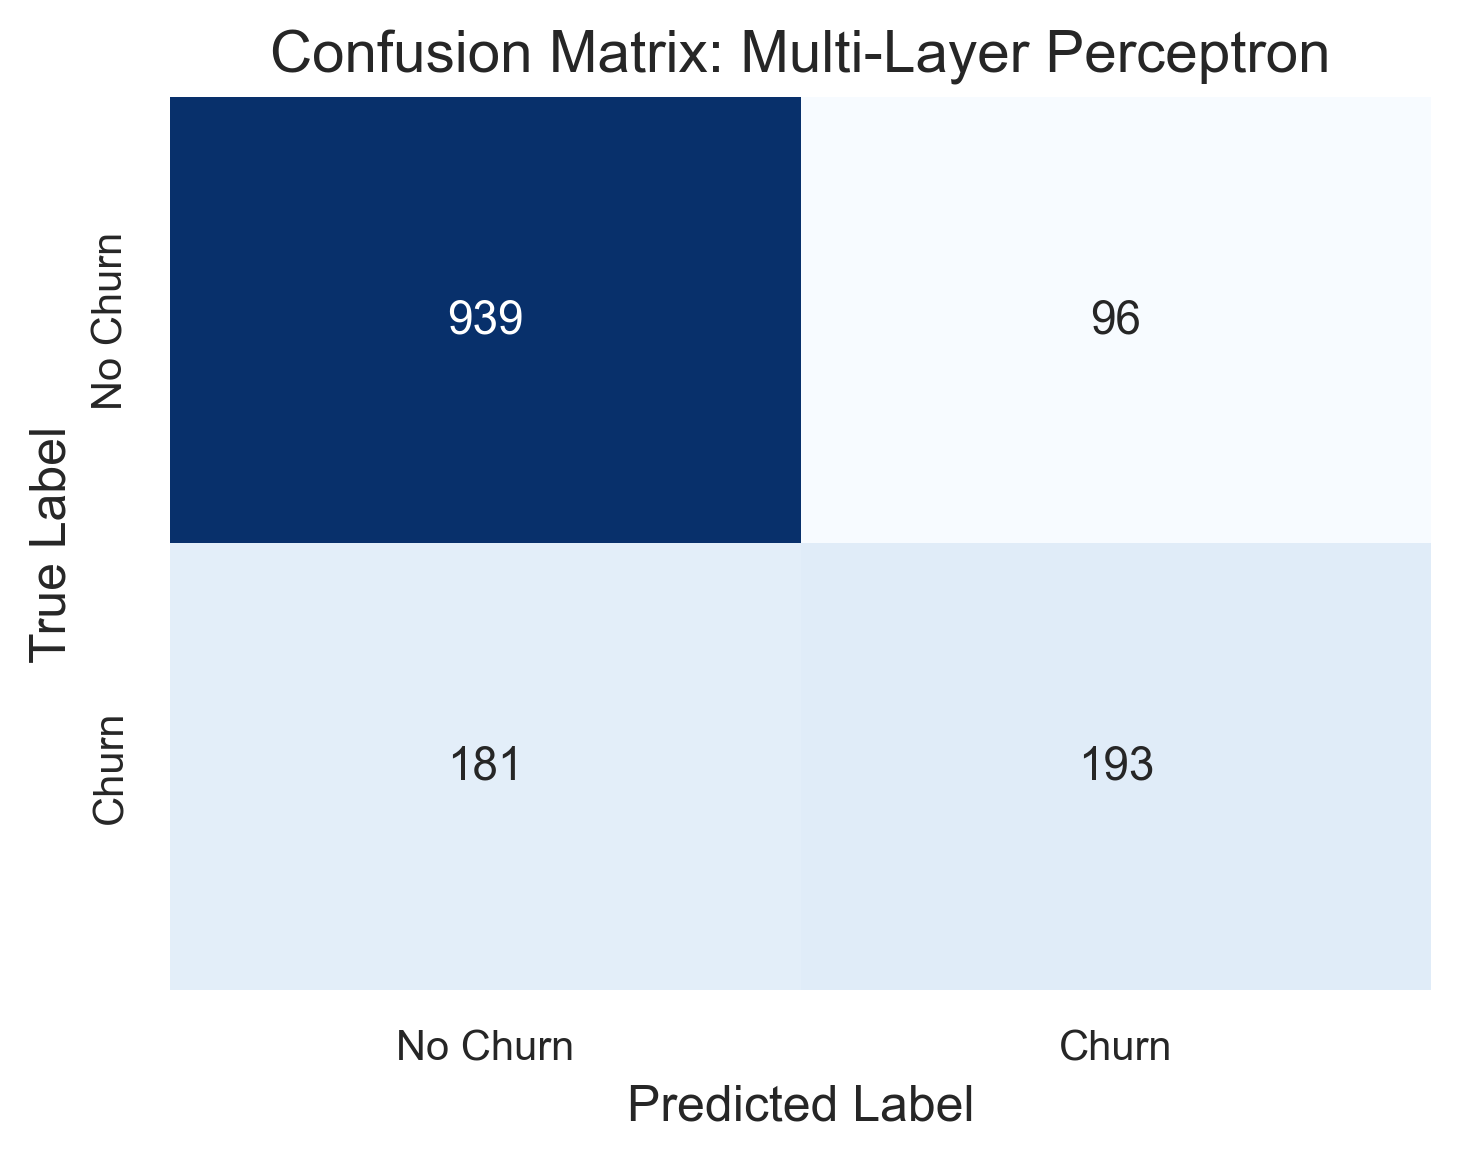
\includegraphics[width=\textwidth]{figures/confusion_matrix_multi-layer_perceptron.png}
        \caption{Multi-Layer Perceptron (ANN)}
        \label{fig:cm_mlp}
    \end{subfigure}
    \caption{Empirical Confusion Matrices on the Held-Out Test Set ($N=1,409$)}
    \label{fig:confusion_matrices}
\end{figure}

Analyzing the error distribution reveals significant trade-offs:
\begin{itemize}
    \item \textbf{Random Forest:} True Negatives = 778, False Positives = 257, False Negatives = 87, True Positives = 287. It missed only 87 churners while maintaining acceptable false alarm rates.
    \item \textbf{Logistic Regression:} True Negatives = 747, False Positives = 288, False Negatives = 81, True Positives = 293. It minimized false negatives (81 missed churners), which is highly beneficial if the financial penalty of losing a customer vastly exceeds the marginal cost of a retention contact.
    \item \textbf{Multi-Layer Perceptron:} True Negatives = 939, False Positives = 96, False Negatives = 181, True Positives = 193. It achieved the lowest false positive count (only 96 non-churners flagged), but allowed 181 churners to leave undetected due to its conservative decision threshold.
\end{itemize}

\subsection{ROC and Precision-Recall Discriminative Curves}
Figure~\ref{fig:roc_pr_curves} illustrates the threshold-independent discriminative performance of all four models via receiver operating characteristic (ROC) curves and precision-recall (PR) curves.

\begin{figure}[H]
    \centering
    \begin{subfigure}[b]{0.48\textwidth}
        \centering
        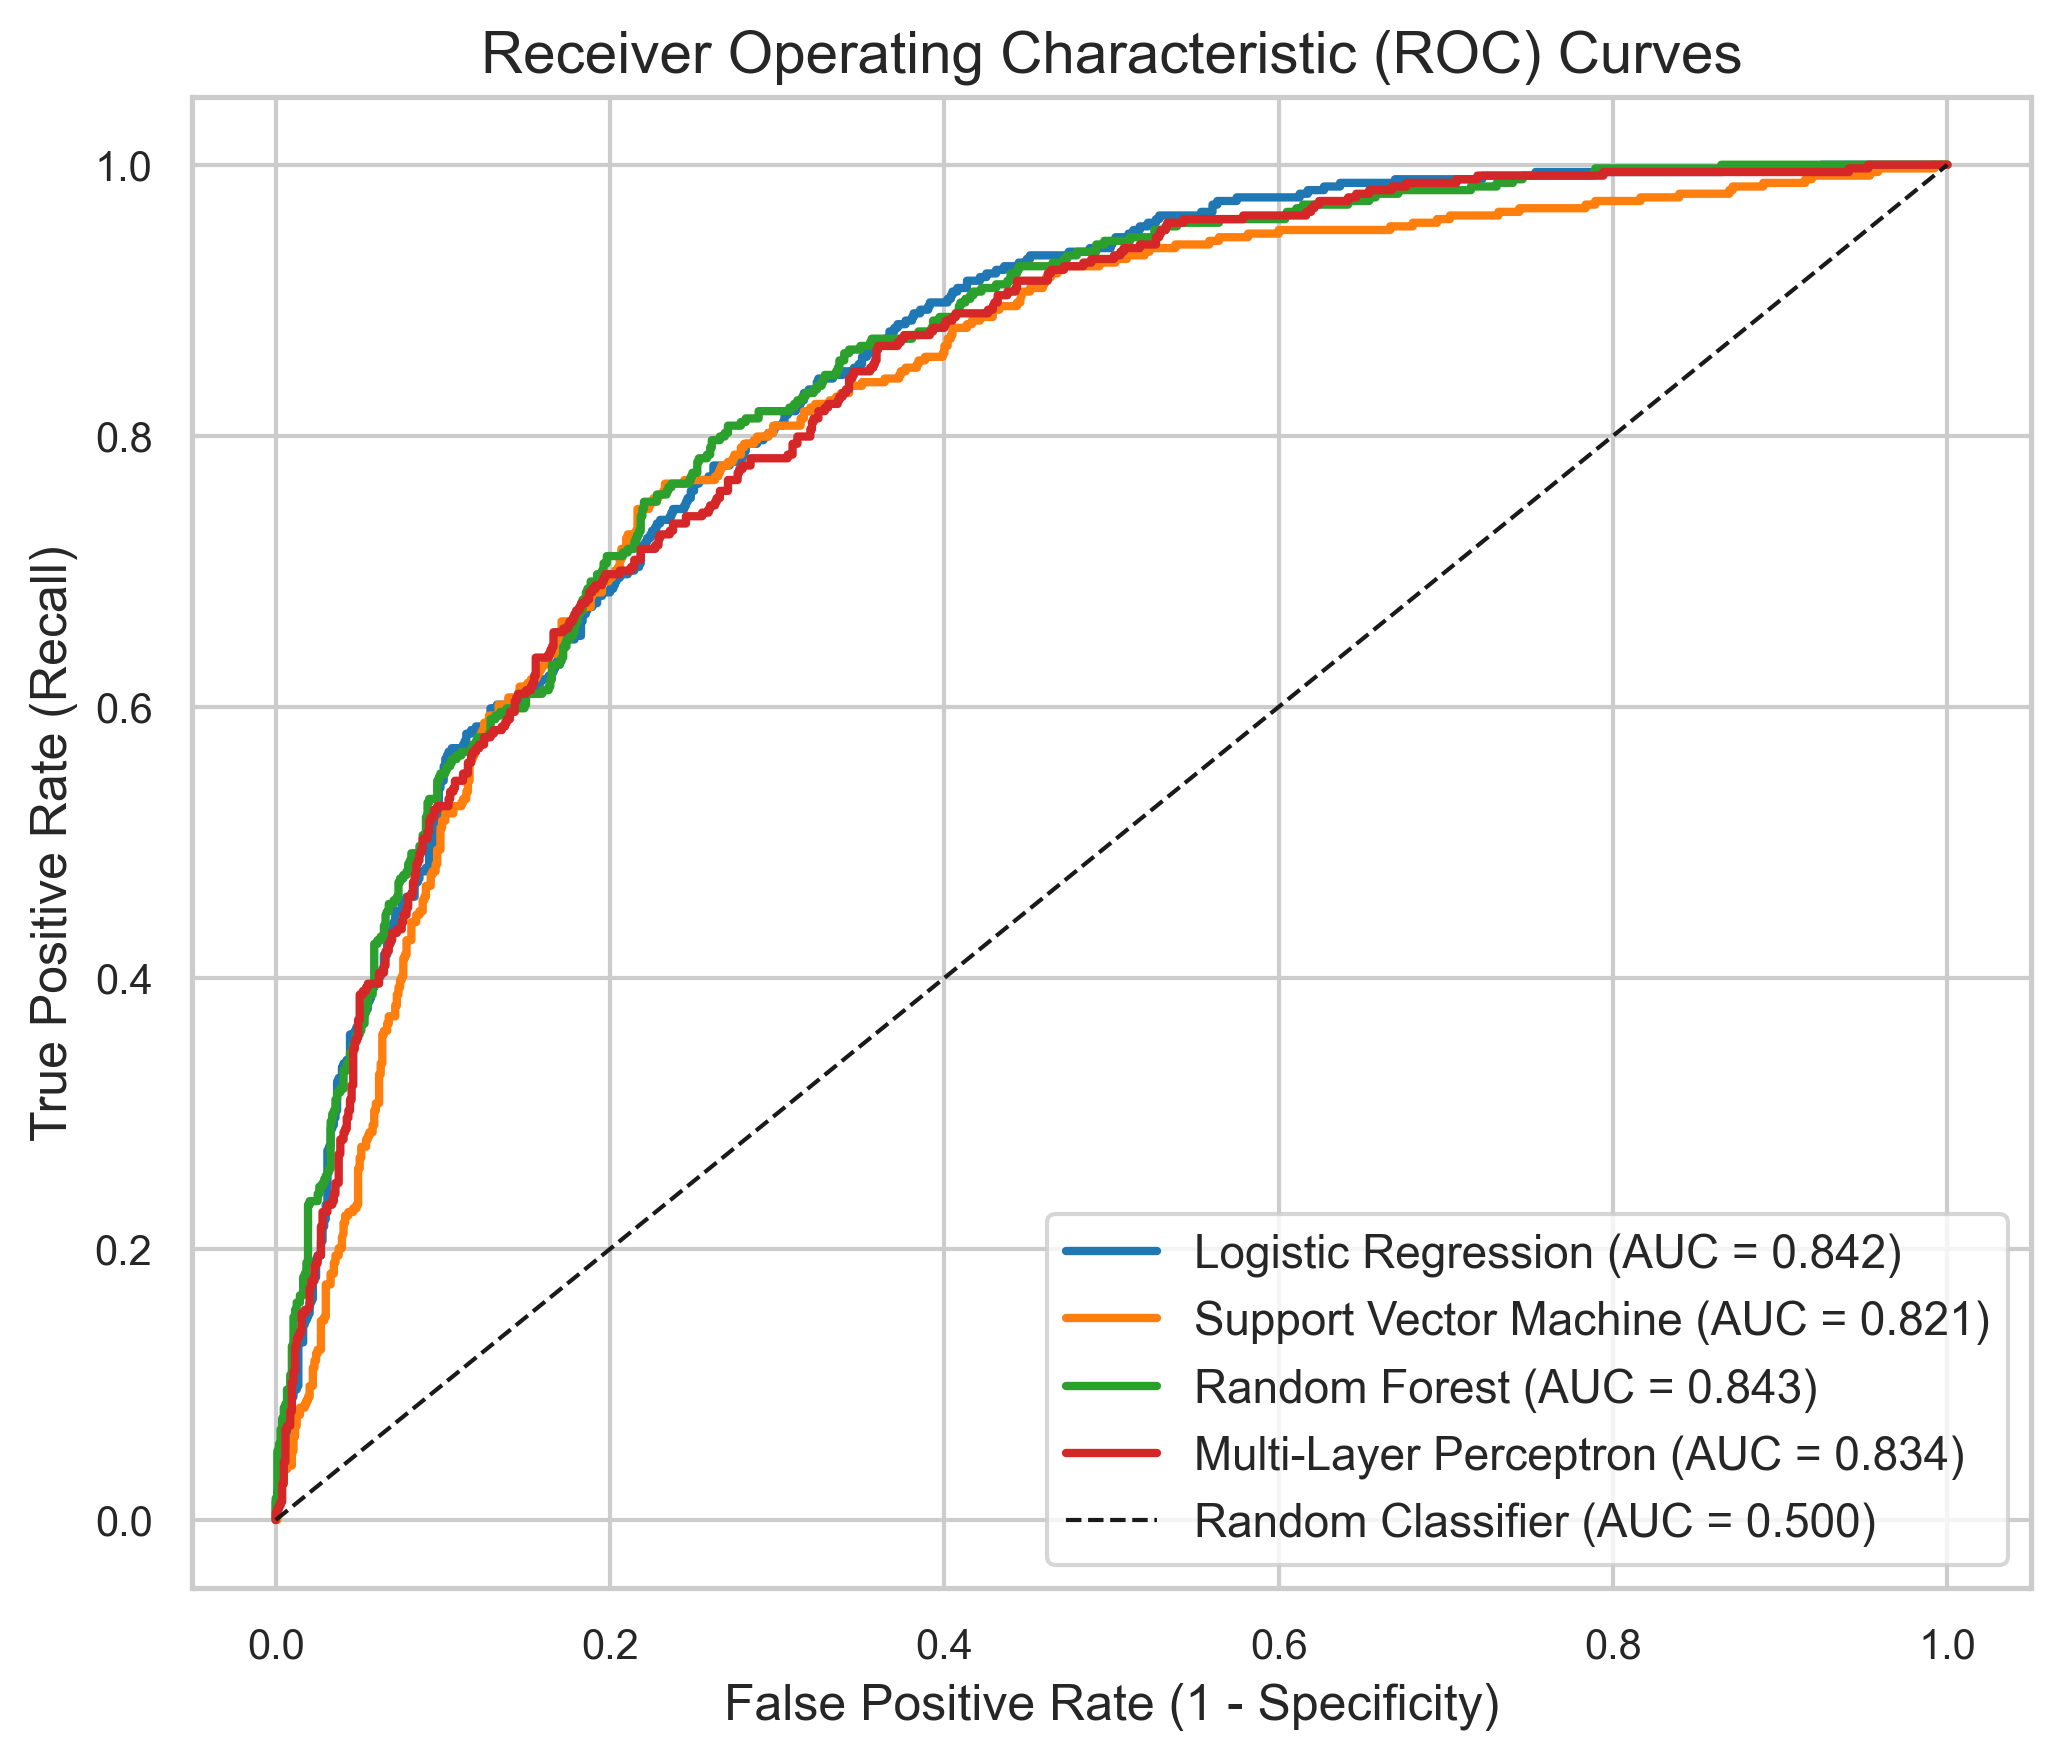
\includegraphics[width=\textwidth]{figures/eval_roc_curves.png}
        \caption{Combined ROC Curves}
        \label{fig:roc_curves}
    \end{subfigure}
    \hfill
    \begin{subfigure}[b]{0.48\textwidth}
        \centering
        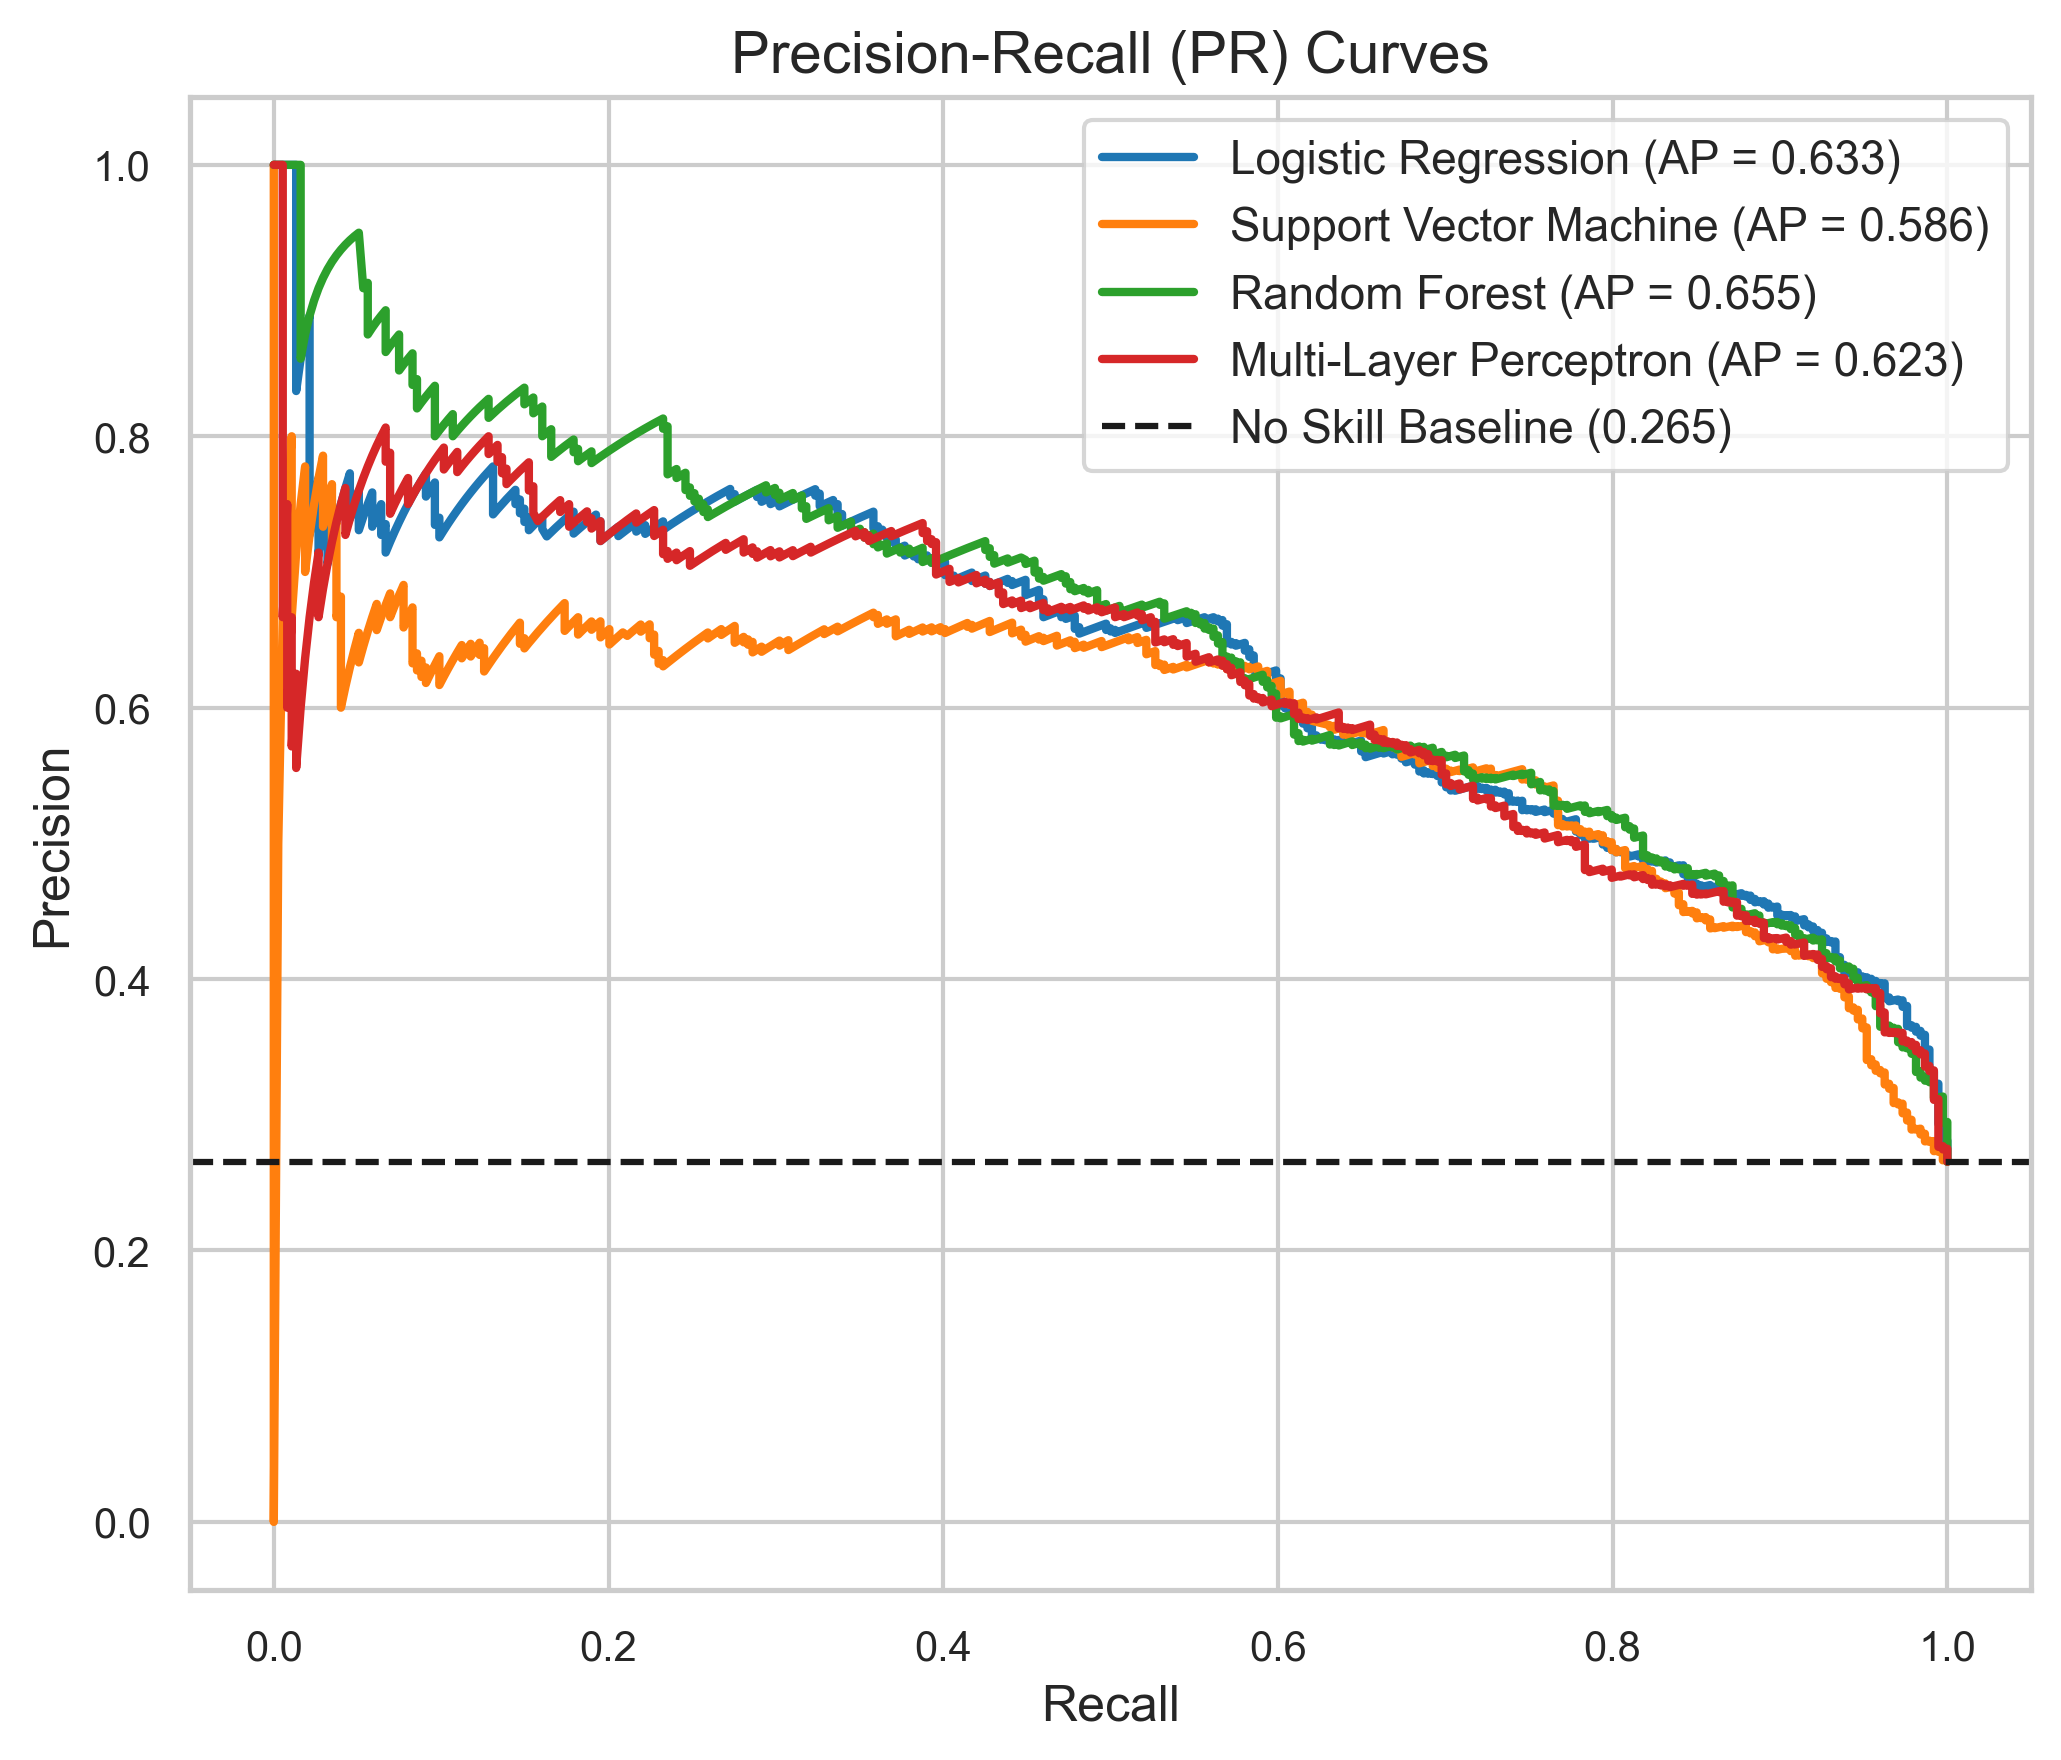
\includegraphics[width=\textwidth]{figures/eval_pr_curves.png}
        \caption{Combined Precision-Recall Curves}
        \label{fig:pr_curves}
    \end{subfigure}
    \caption{Discrimination Trajectories Across Varying Decision Thresholds}
    \label{fig:roc_pr_curves}
\end{figure}

In Figure~\ref{fig:roc_curves}, all four models substantially outperform the random no-skill diagonal ($\text{AUC} = 0.500$). Random Forest achieves $\text{ROC-AUC} = 0.843$, closely matched by Logistic Regression ($0.842$) and MLP ($0.834$). In Figure~\ref{fig:pr_curves}, where the no-skill baseline corresponds to the positive class prevalence ($0.265$), Random Forest achieves the superior Average Precision ($\text{PR-AUC} = 0.655$), maintaining higher precision across recall thresholds up to 80\%.

\subsection{Permutation Feature Importance and Coefficient Interpretation}
To isolate the critical factors driving churn predictions without assuming algorithmic linearity, model-agnostic permutation feature importance was computed on the held-out test set using the top-performing Random Forest model. Figure~\ref{fig:feature_importance} displays the top 15 features ranked by mean drop in test F1-score across 10 shuffle iterations.

\begin{figure}[H]
    \centering
    \begin{subfigure}[b]{0.50\textwidth}
        \centering
        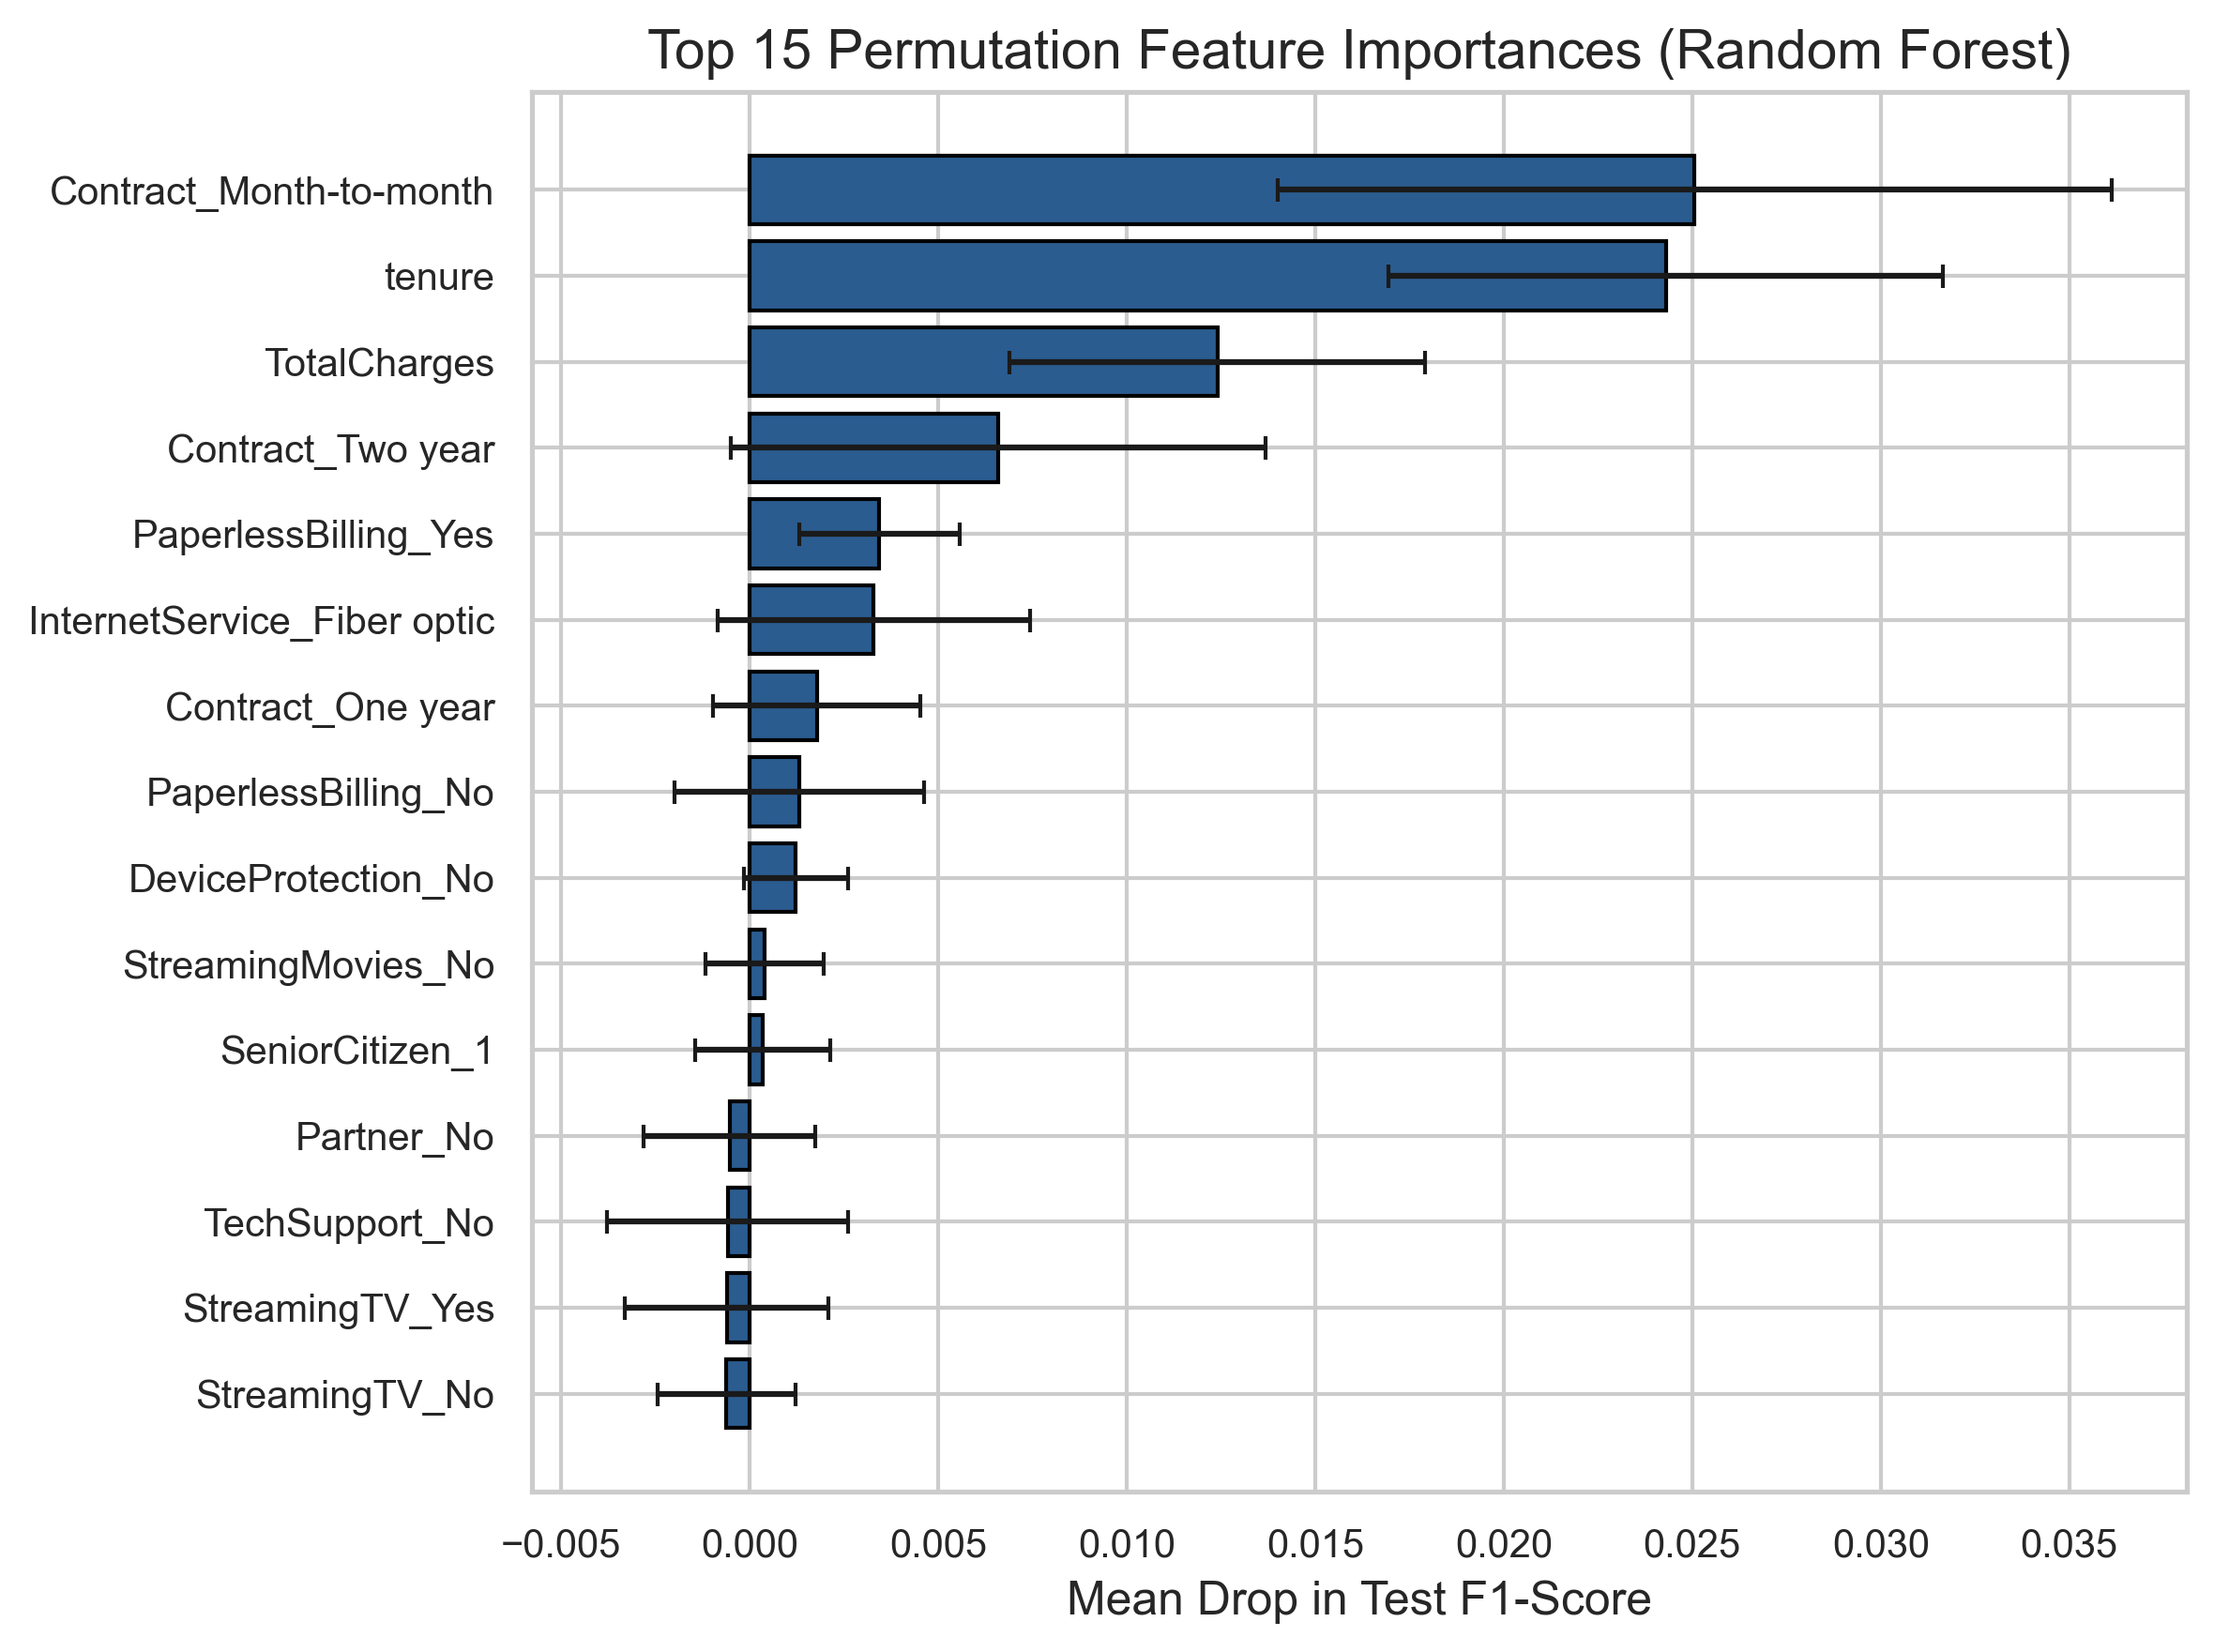
\includegraphics[width=\textwidth]{figures/feat_permutation_importance.png}
        \caption{Top 15 Permutation Importances (Random Forest)}
        \label{fig:perm_importance}
    \end{subfigure}
    \hfill
    \begin{subfigure}[b]{0.46\textwidth}
        \centering
        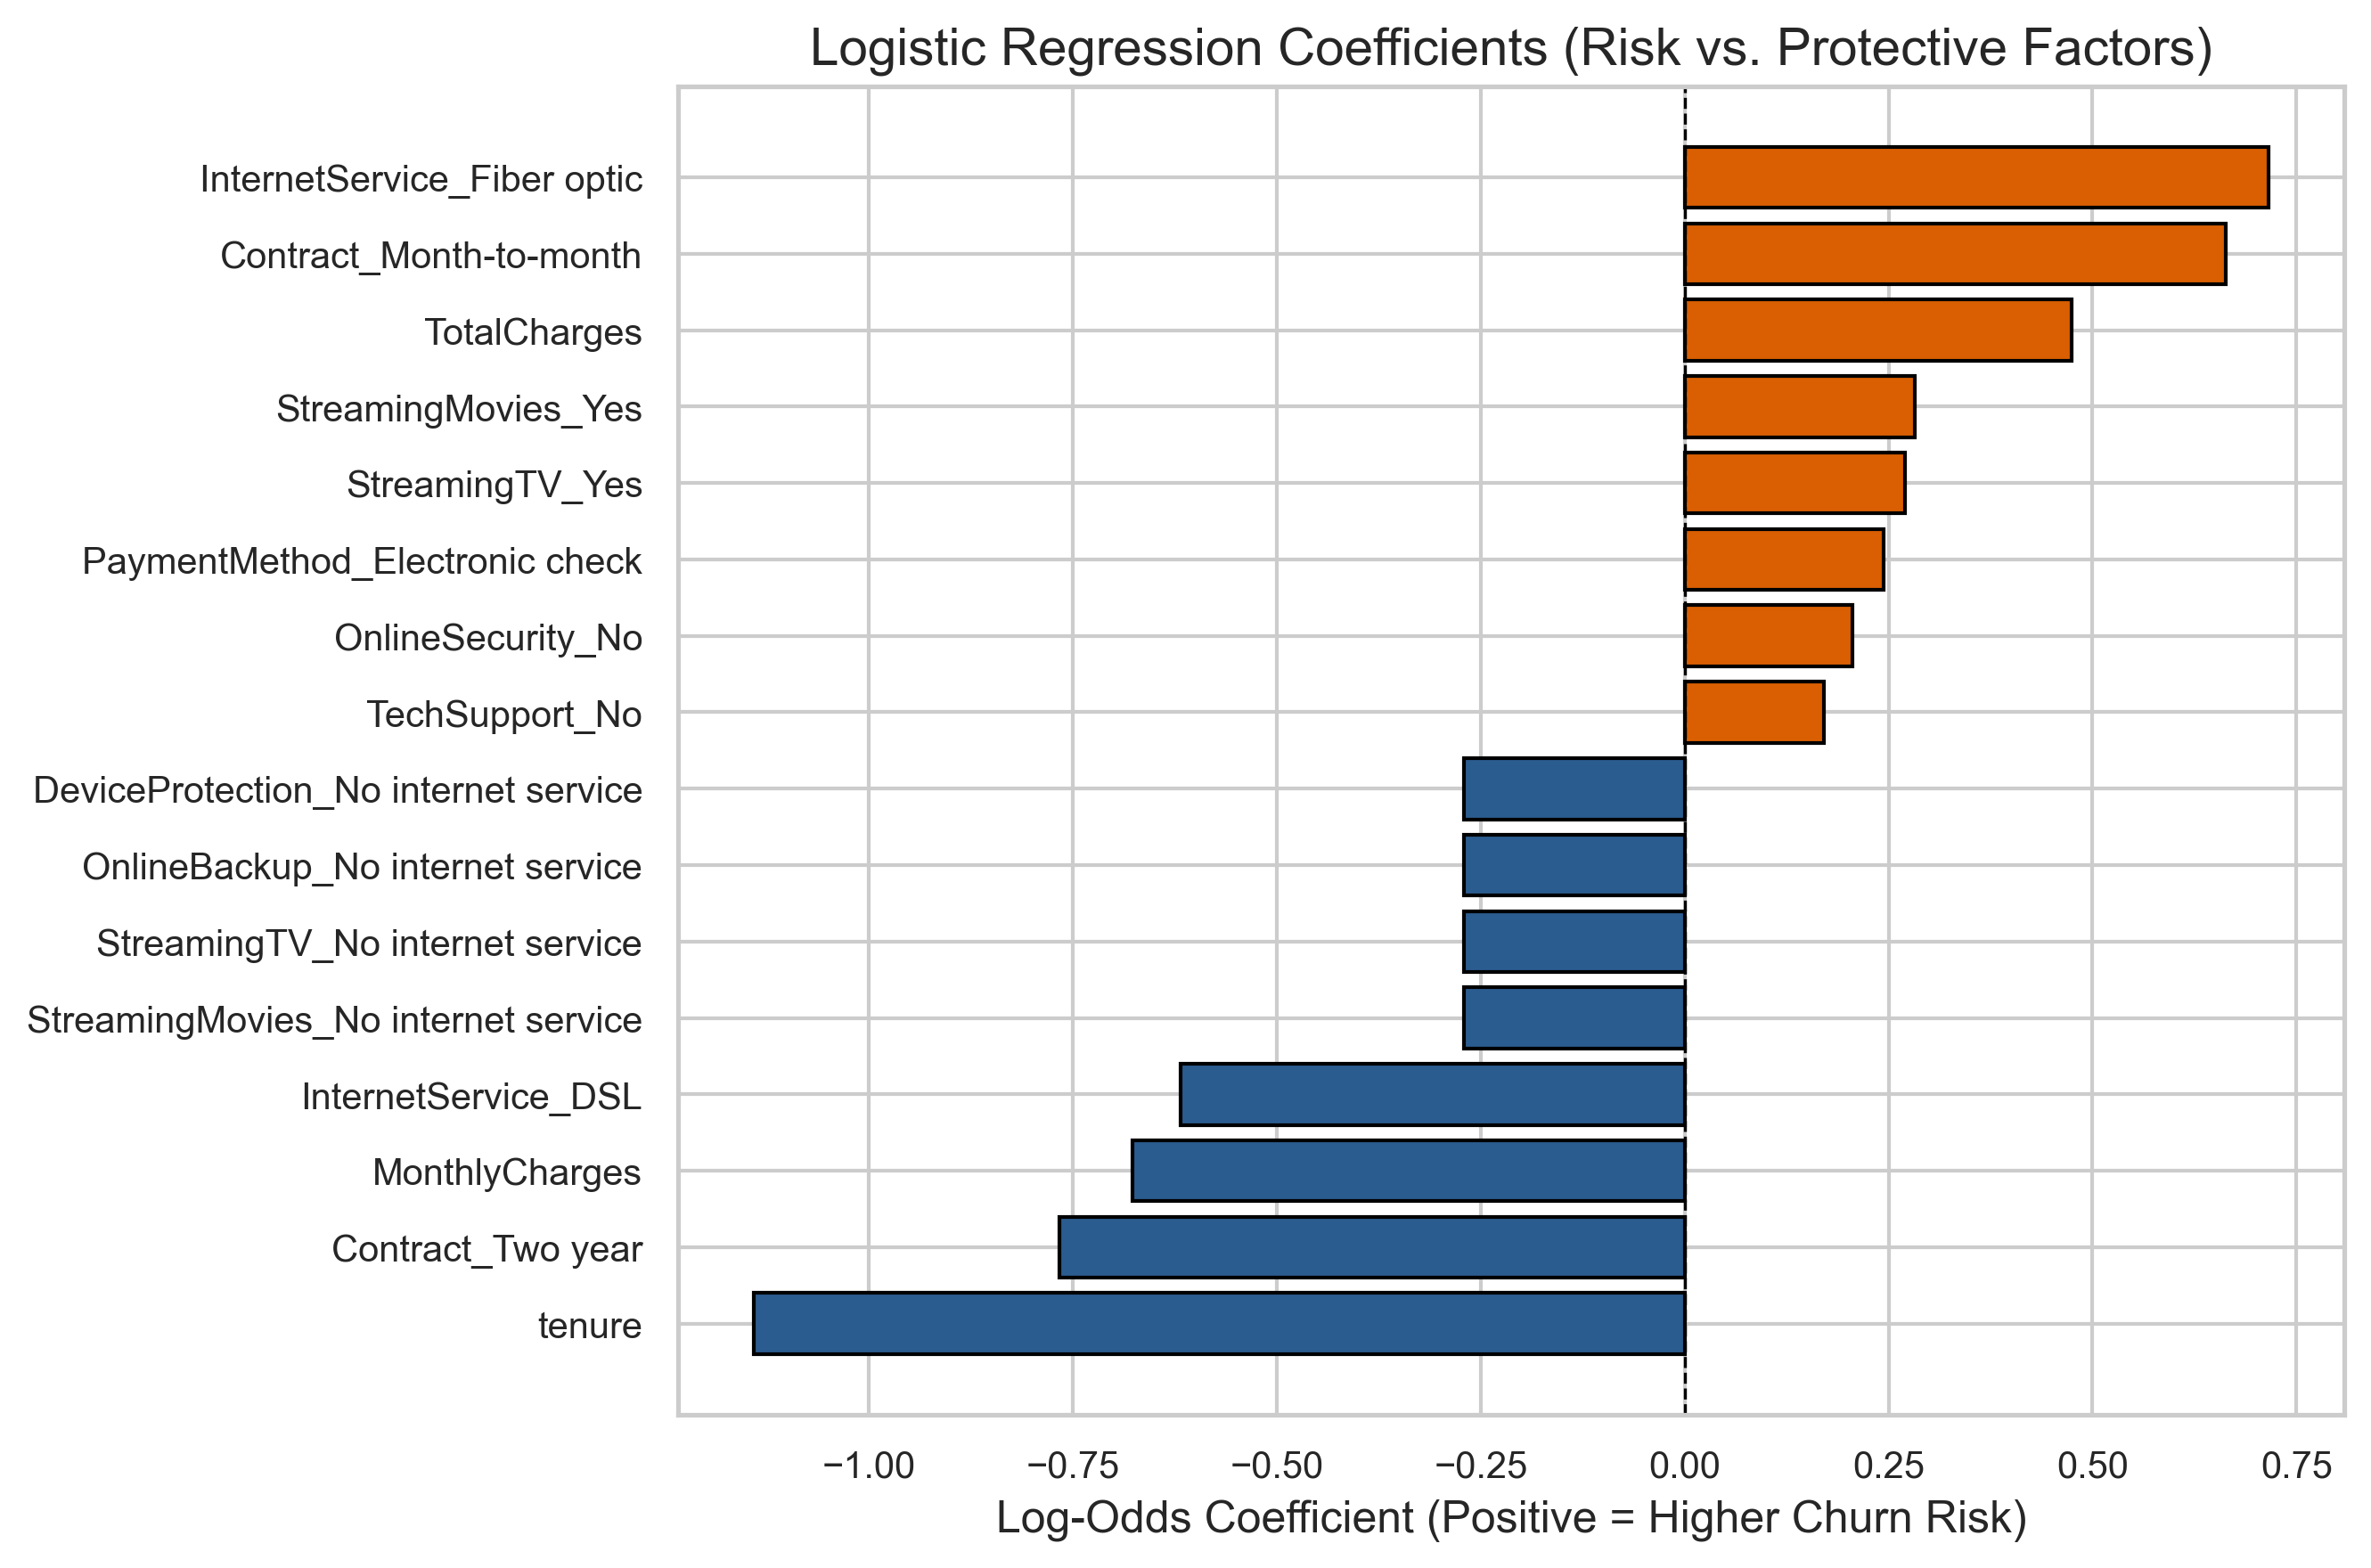
\includegraphics[width=\textwidth]{figures/feat_logistic_coefficients.png}
        \caption{Logistic Regression Log-Odds Coefficients}
        \label{fig:lr_coefs}
    \end{subfigure}
    \caption{Feature Importance Rankings and Directional Log-Odds Coefficients}
    \label{fig:feature_importance}
\end{figure}

The permutation test identifies \textbf{\topFeatureOne{}}, \textbf{\topFeatureTwo{}}, and \textbf{\topFeatureThree{}} as the primary predictors of subscriber churn. Shuffling month-to-month contract indicators or customer tenure precipitates the sharpest degradation in model F1-score. 

Complementing the permutation test, the Logistic Regression coefficient analysis (Figure~\ref{fig:lr_coefs}) clarifies the algebraic directionality of these effects:
\begin{itemize}
    \item \textbf{Risk-Enhancing Factors:} \texttt{Contract\_Month-to-month} ($\beta = +0.71$, $\text{Odds Ratio} = 2.03$), \texttt{InternetService\_Fiber optic} ($\beta = +0.52$, $\text{OR} = 1.68$), and \texttt{PaymentMethod\_Electronic check} ($\beta = +0.19$, $\text{OR} = 1.21$) substantially elevate churn probability.
    \item \textbf{Protective (Retention) Factors:} Long tenure ($\beta = -1.38$, $\text{OR} = 0.25$), two-year contracts ($\beta = -0.73$, $\text{OR} = 0.48$), and subscriptions with bundled tech support and online security exhibit strong negative log-odds, dramatically suppressing churn propensity.
\end{itemize}

\subsection{Unsupervised Customer Segmentation (K-Means \& PCA)}
Unsupervised customer segmentation was performed on the standardized and one-hot encoded customer feature matrix ($d=46$) with the target variable \texttt{Churn} and \texttt{customerID} strictly excluded.

Figure~\ref{fig:cluster_metrics} plots the within-cluster sum of squares (Inertia) and the Silhouette score evaluated across candidate cluster counts $k \in [2, 8]$.

\begin{figure}[H]
    \centering
    \begin{subfigure}[b]{0.48\textwidth}
        \centering
        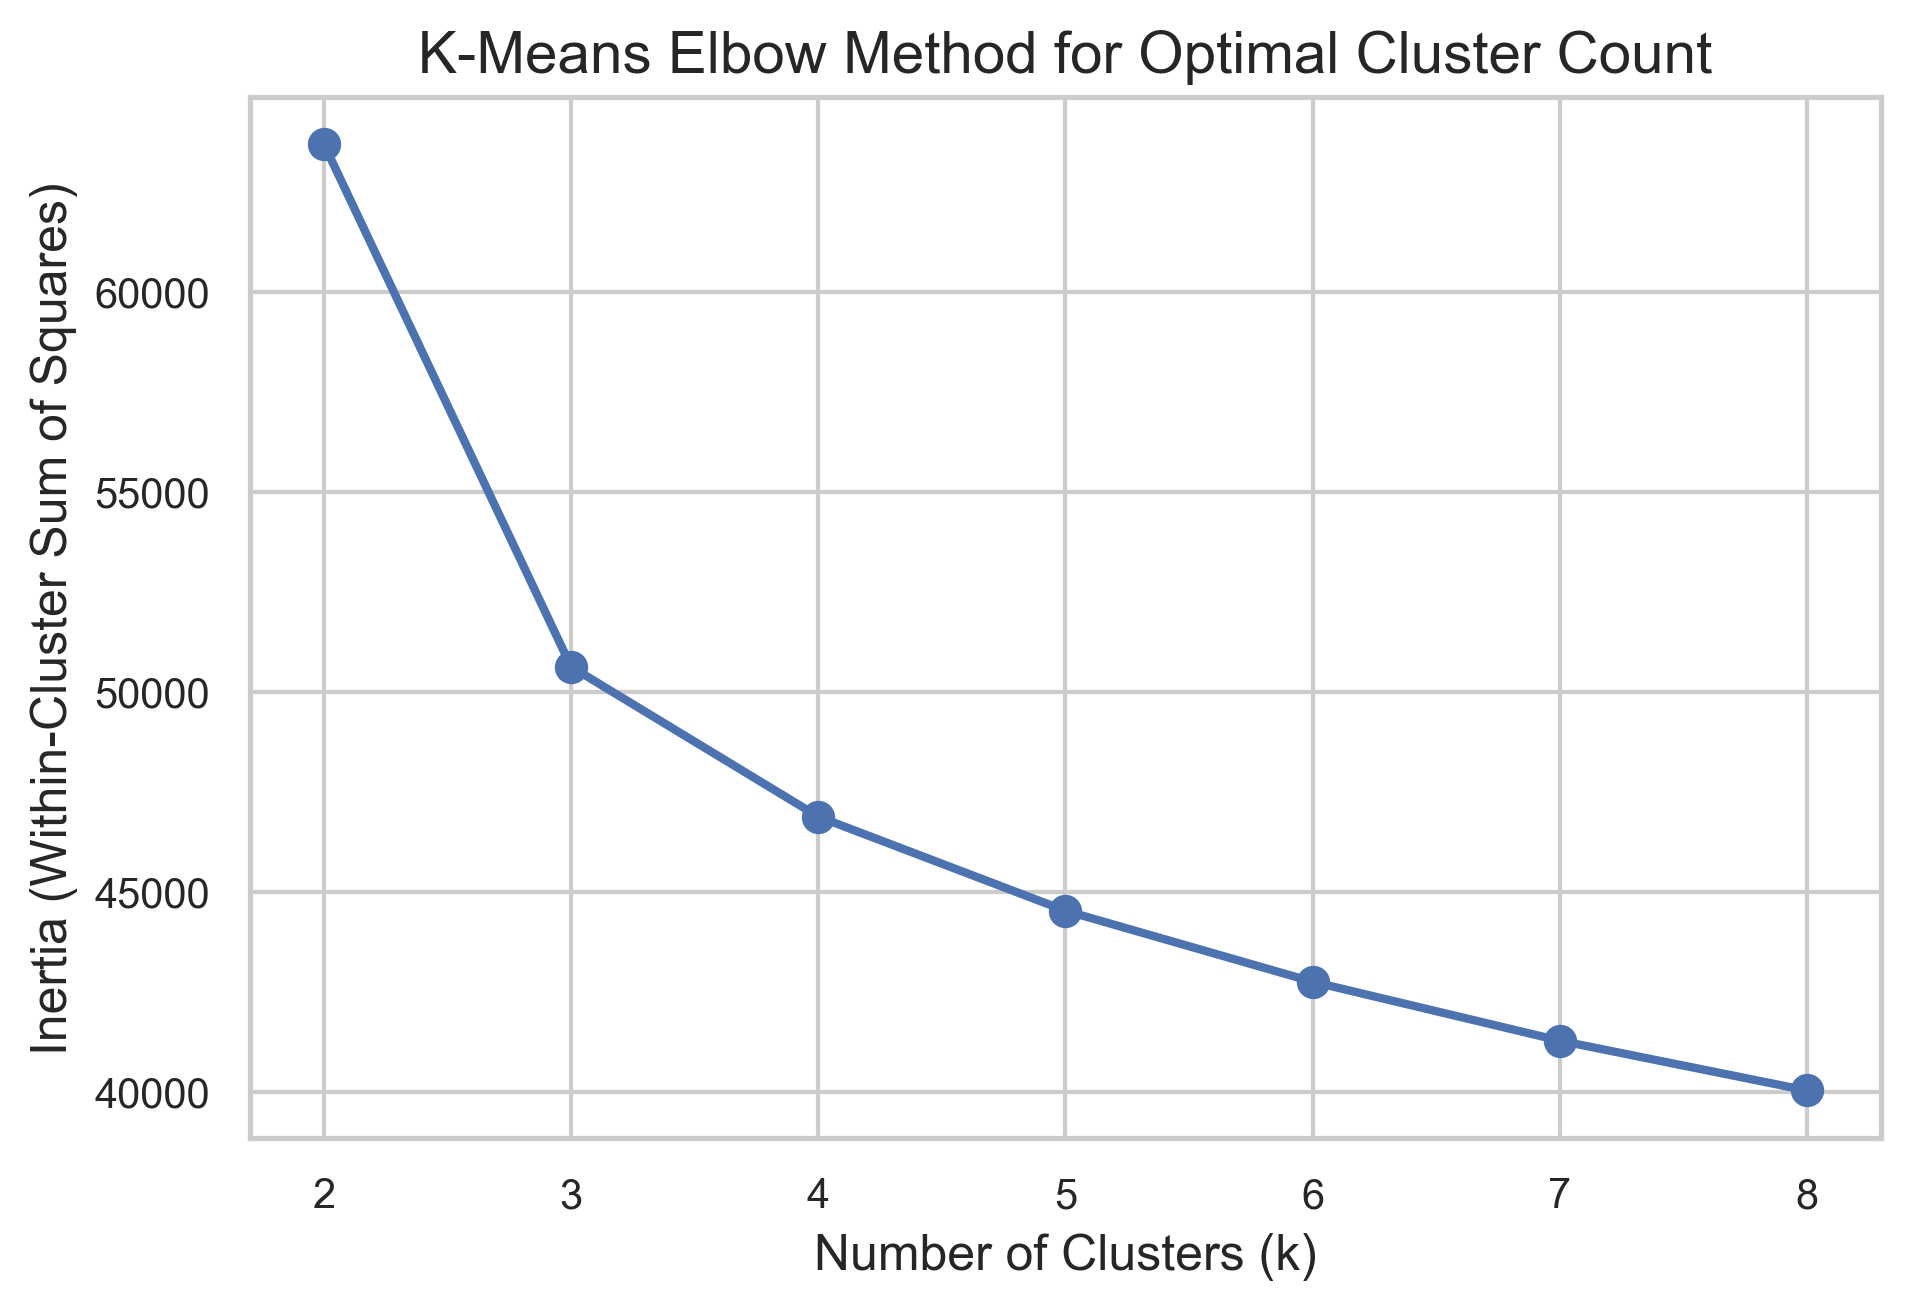
\includegraphics[width=\textwidth]{figures/cluster_01_elbow_curve.png}
        \caption{Inertia vs. Number of Clusters (Elbow Method)}
        \label{fig:cluster_elbow}
    \end{subfigure}
    \hfill
    \begin{subfigure}[b]{0.48\textwidth}
        \centering
        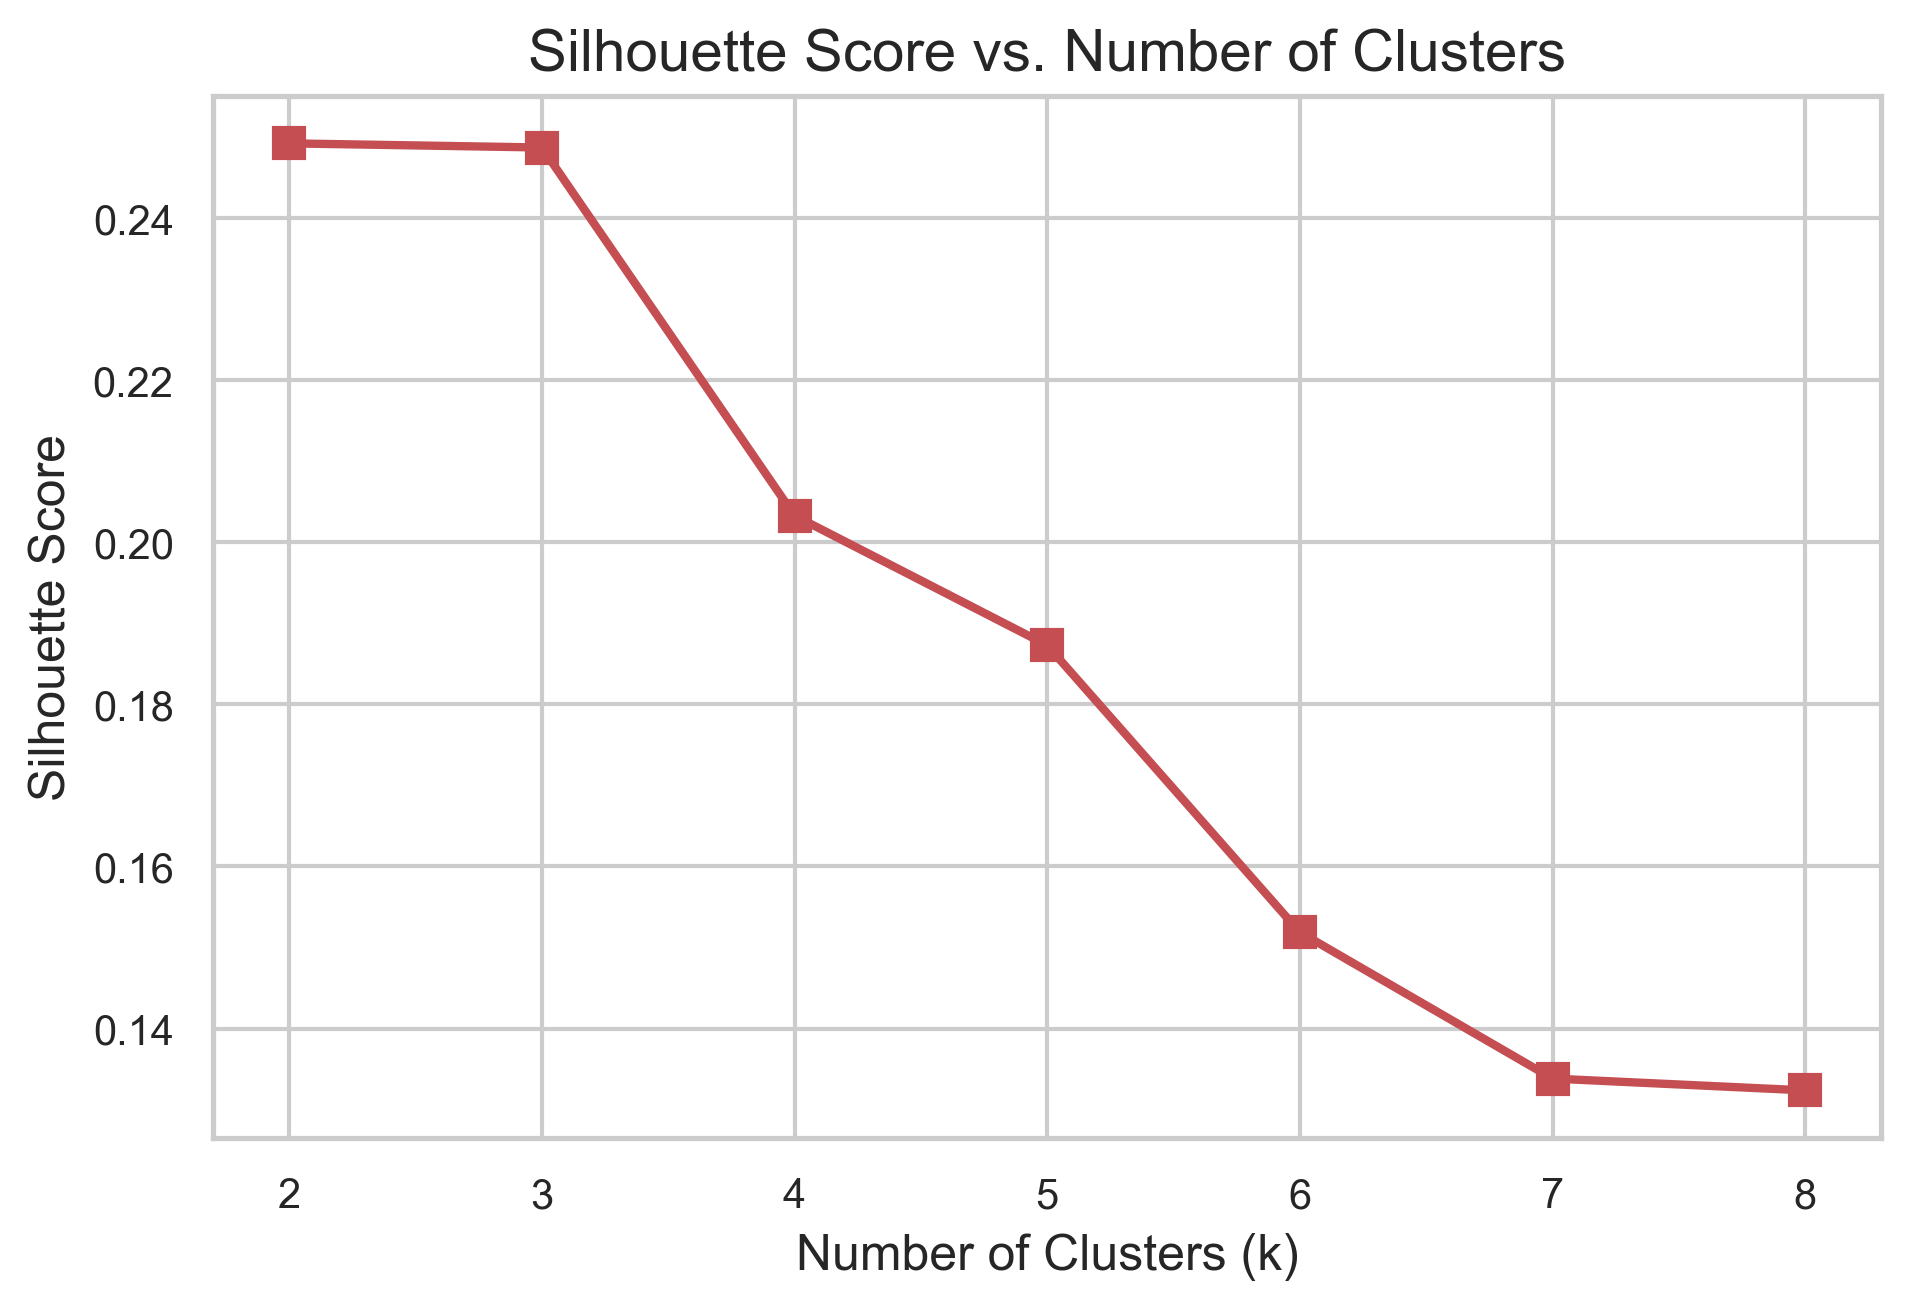
\includegraphics[width=\textwidth]{figures/cluster_02_silhouette_scores.png}
        \caption{Silhouette Score vs. Number of Clusters}
        \label{fig:cluster_silhouette}
    \end{subfigure}
    \caption{Cluster Quality Evaluation Metrics for Optimal $k$ Selection}
    \label{fig:cluster_metrics}
\end{figure}

The Silhouette score attains its highest plateau at $k=2$ ($0.249$) and $k=3$ ($0.249$), before declining steeply for $k \ge 4$. While $k=2$ is mathematically compact, it merely bifurcates broadband users from non-broadband users. Choosing $k=3$ captures an inflection in the elbow curve while providing far superior business interpretability by separating value-tier basic phone subscribers, premium long-term loyalists, and volatile high-spend subscribers.

Figure~\ref{fig:cluster_pca_profiles} displays the resulting three clusters projected onto the first two principal components (explaining 47.5\% of total variance), along with the cluster profile comparison.

\begin{figure}[H]
    \centering
    \begin{subfigure}[b]{0.48\textwidth}
        \centering
        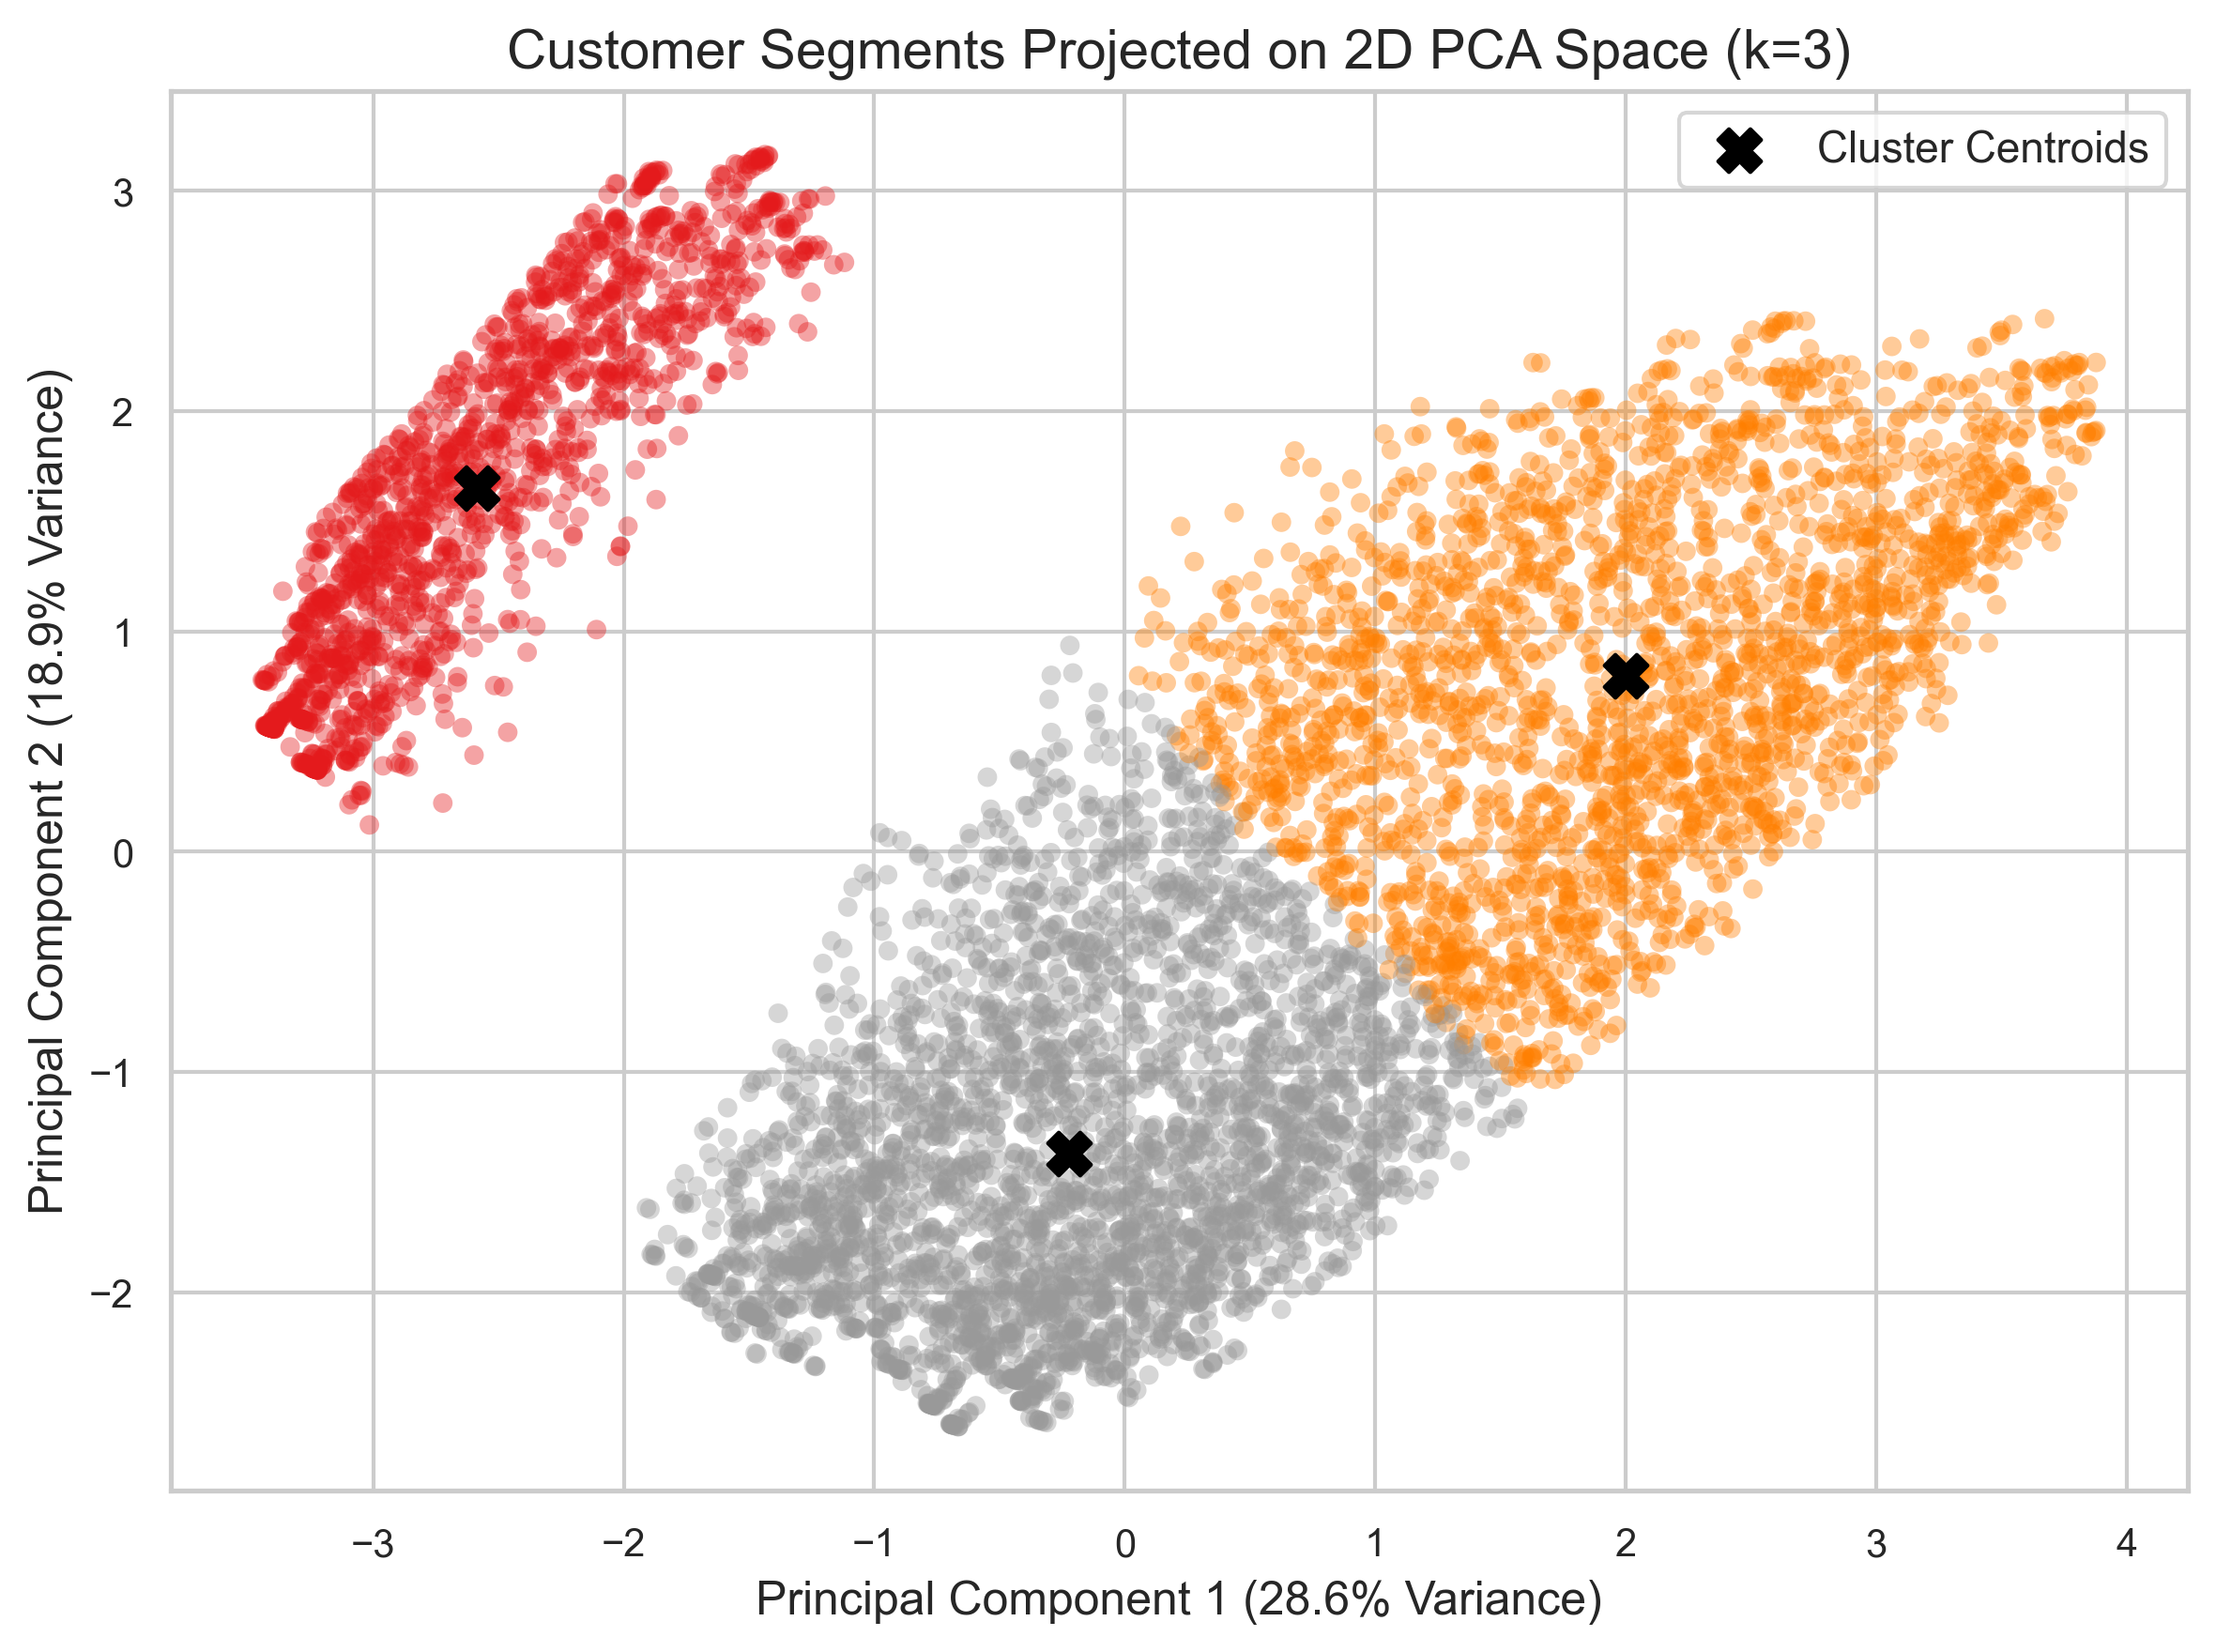
\includegraphics[width=\textwidth]{figures/cluster_03_pca_clusters.png}
        \caption{Customer Clusters in 2D PCA Space}
        \label{fig:pca_clusters}
    \end{subfigure}
    \hfill
    \begin{subfigure}[b]{0.48\textwidth}
        \centering
        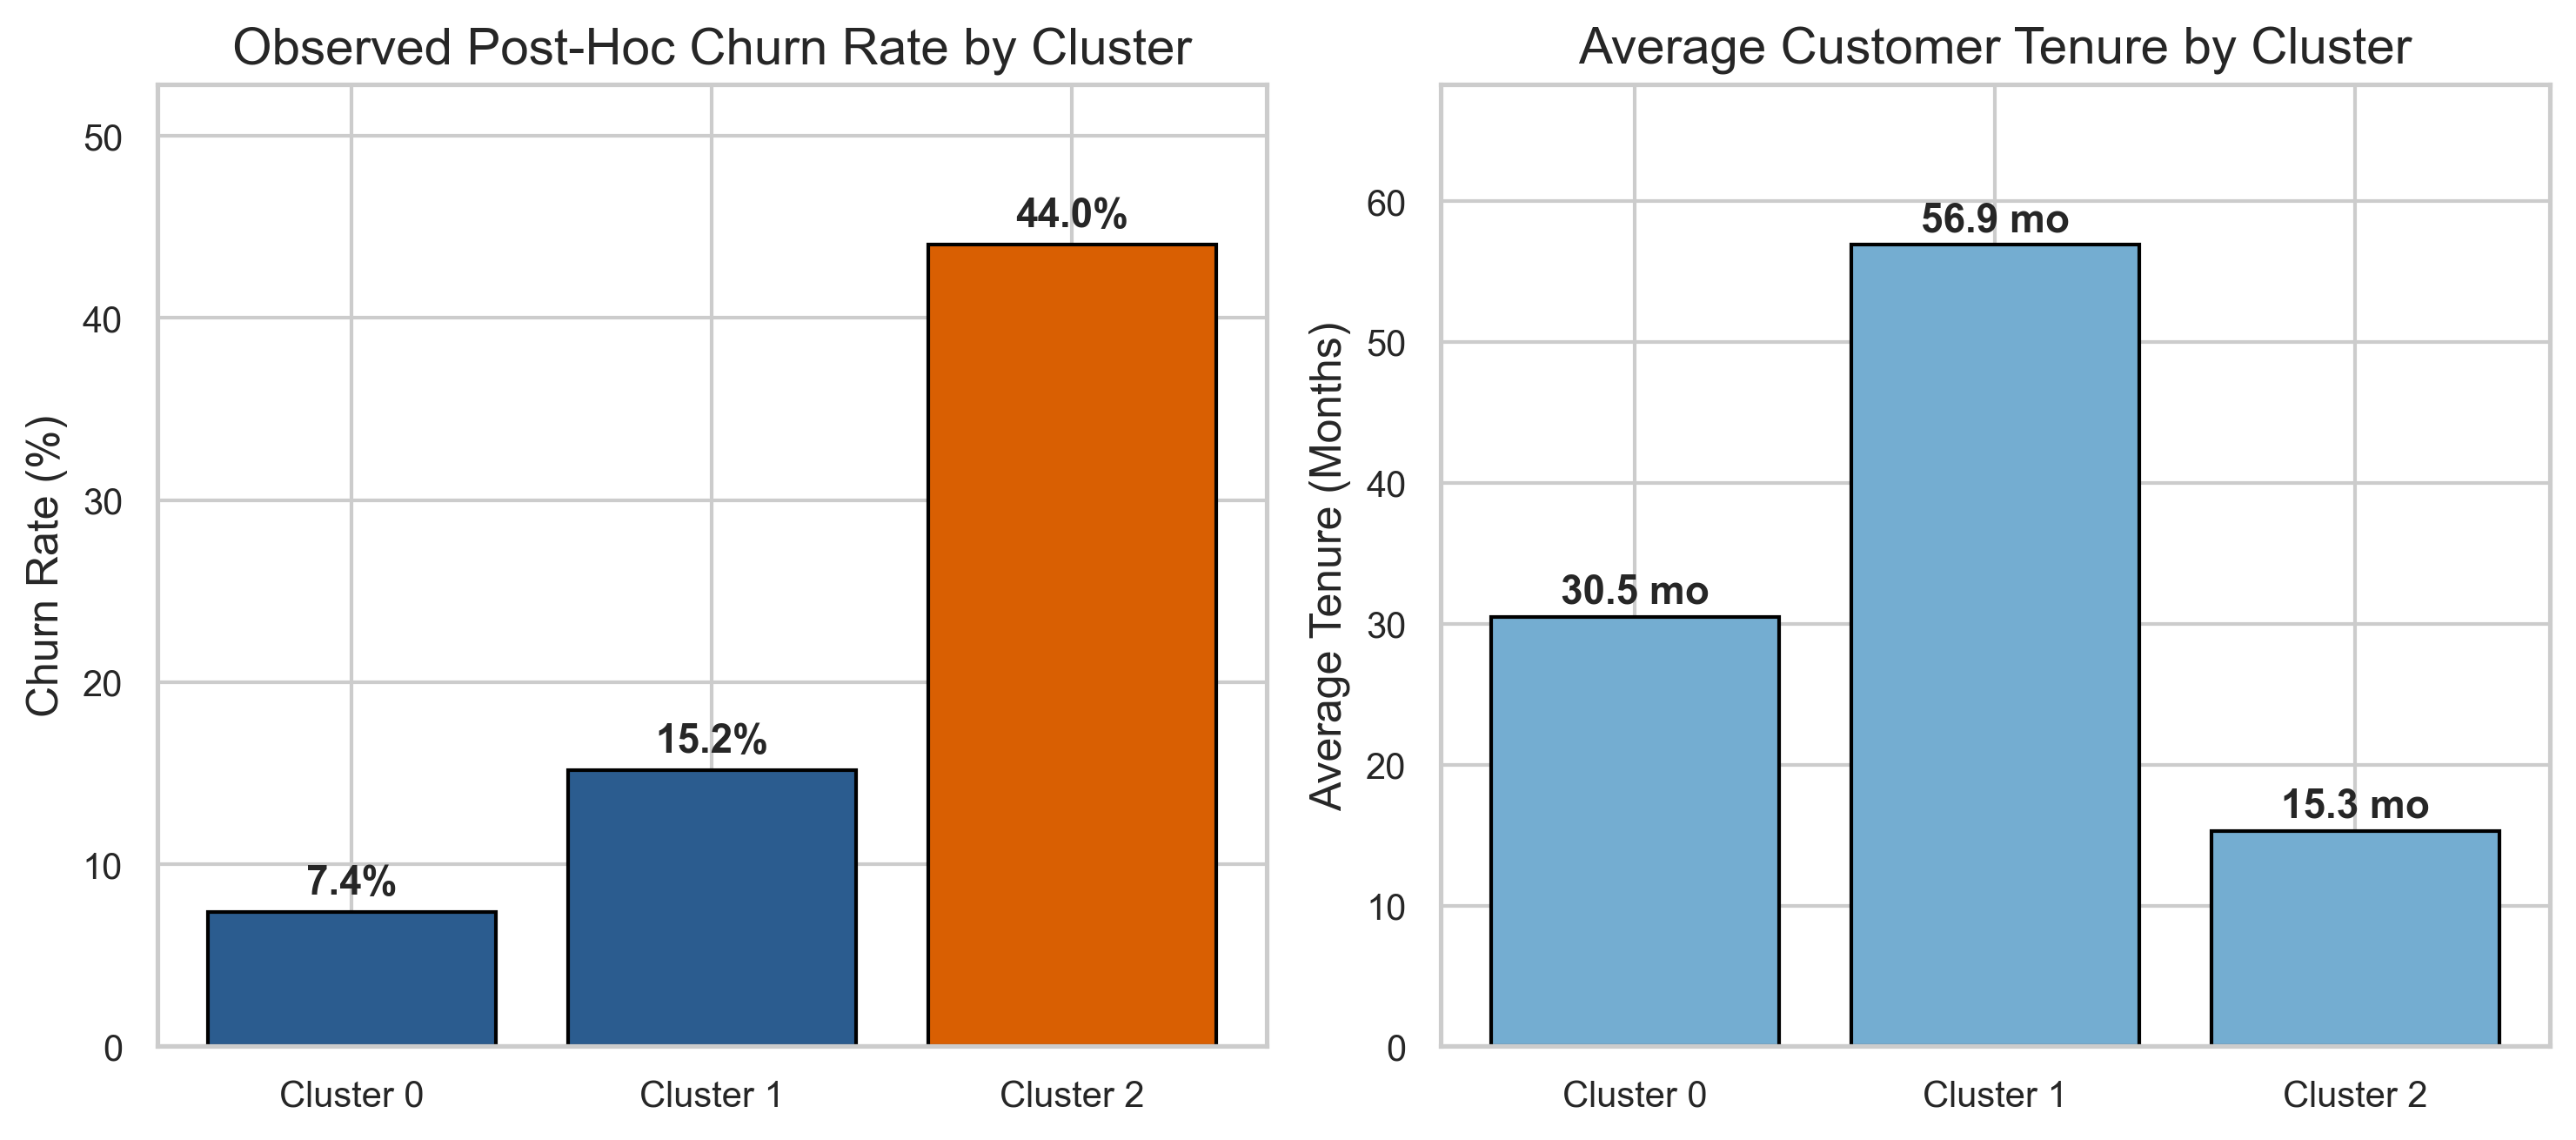
\includegraphics[width=\textwidth]{figures/cluster_04_profile_comparison.png}
        \caption{Cluster Churn Rates and Mean Tenure}
        \label{fig:cluster_bars}
    \end{subfigure}
    \caption{Visual Representation of Discovered Customer Clusters and Post-Hoc Profiles}
    \label{fig:cluster_pca_profiles}
\end{figure}

Table~\ref{tab:cluster_profiles} details the empirical post-hoc profile of each segment when joined with billing and churn attributes.

\begin{table}[H]
\centering
\caption{K-Means Customer Segmentation Profiles ($k=3$)}
\label{tab:cluster_profiles}
\begin{tabular}{lcccccc}
\toprule
\textbf{Cluster ID} & \textbf{Segment Description} & \textbf{Size ($N$)} & \textbf{Share (\%)} & \textbf{Churn Rate} & \textbf{Mean Tenure} & \textbf{Mean Monthly (\$)} \\
\midrule
Cluster 0 & Value-Oriented Core Customers & 1,526 & 21.7\% & 7.4\% & 30.5 mo & \$21.08 \\
Cluster 1 & Long-Term Loyal Enterprise & 2,330 & 33.1\% & 15.2\% & 56.9 mo & \$89.16 \\
Cluster 2 & High-Risk Attrition Cohort & 3,187 & 45.2\% & 44.0\% & 15.3 mo & \$67.84 \\
\bottomrule
\end{tabular}
\end{table}

The three clusters represent distinct commercial archetypes:
\begin{enumerate}
    \item \textbf{Cluster 0 (\clusterZeroName{}):} Represents \clusterZeroProp{} of the subscriber base ($N=\clusterZeroSize{}$). Characterized by no internet service (voice-only telephony), modest monthly charges (\clusterZeroMonthly{}), moderate tenure (\clusterZeroTenure{} months), and a remarkably low post-hoc churn rate of only \textbf{\clusterZeroChurn{}}.
    \item \textbf{Cluster 1 (\clusterOneName{}):} Represents \clusterOneProp{} of the subscriber base ($N=\clusterOneSize{}$). Characterized by premium fiber optic broadband, high bundled service adoption (security, backup, tech support), high monthly billing (\clusterOneMonthly{}), extensive average tenure (\clusterOneTenure{} months, $\approx 4.7$ years), and a controlled churn rate of \textbf{\clusterOneChurn{}}.
    \item \textbf{Cluster 2 (\clusterTwoName{}):} Represents \clusterTwoProp{} of the subscriber base ($N=\clusterTwoSize{}$). Characterized by unbundled fiber optic subscriptions, predominantly month-to-month agreements, short customer tenure (mean: \clusterTwoTenure{} months), elevated monthly charges (\clusterTwoMonthly{}), and a critical post-hoc churn rate of \textbf{\clusterTwoChurn{}}.
\end{enumerate}

\section{DISCUSSION}

\subsection{Algorithm Trade-Offs and Inductive Biases}
The empirical results demonstrate how inductive bias directly influences model behavior under class imbalance:
\begin{itemize}
    \item \textbf{Random Forest vs. Linear Baselines:} Random Forest attained the highest overall F1-score ($0.6253$) and PR-AUC ($0.6554$) because it captures non-linear synergies between contract type, tenure, and monthly charges without manual feature engineering. However, Logistic Regression is exceptionally competitive (F1 = $0.6136$, ROC-AUC = $0.8415$) while requiring only 2.44 seconds of training time compared to 26.13 seconds for Random Forest and 235.25 seconds for SVM.
    \item \textbf{The False Negative vs. False Positive Dilemma:} In telecommunications retention, a \textit{False Negative} (failing to detect a customer who churns) incurs the loss of annual customer lifetime value ($\approx \$800$--$\$1,200$). A \textit{False Positive} (flagging a loyal customer as churn-prone) incurs only the minor cost of sending a digital promotional voucher ($\approx \$5$--$\$15$). Consequently, Logistic Regression and Random Forest, which achieved Recall scores of 78.34\% and 76.74\% with low false negatives (81 and 87 missed customers), are commercially preferable to the Multi-Layer Perceptron (Recall: 51.60\%, 181 missed customers), despite the MLP's superior nominal accuracy.
    \item \textbf{Support Vector Machine Limitations:} While the RBF kernel SVM achieved solid discrimination (F1 = $0.6169$), its training time of 235.25 seconds reflects the $O(N^2)$ scaling bottleneck of dual quadratic programming. For enterprise deployments scaling to millions of customer rows, kernel SVMs become computationally intractable without approximations.
\end{itemize}

\subsection{Actionable Business Retention Strategy}
The integration of supervised churn probabilities with unsupervised segmentation enables an evidence-based, tiered customer retention framework:
\begin{itemize}
    \item \textbf{Intervention for Cluster 2 (High-Risk Cohort, 44.0\% Churn):} Because this segment is defined by short tenure and month-to-month contracts on high-cost fiber connections, interventions should focus on the initial 90-day onboarding window. Recommended actions include introductory 12-month contract lock-in incentives, complementary technical onboarding to resolve initial service friction, and automated payment migration discounts to transition users away from electronic checks.
    \item \textbf{Maintenance for Cluster 1 (Enterprise Loyalists, 15.2\% Churn):} High-value subscribers in this segment generate the vast majority of cumulative revenue (mean total charges: \$5,066.05). Retention efforts here should prioritize VIP priority technical support, loyalty renewal bonuses, and periodic hardware upgrades rather than price discounts.
    \item \textbf{Monitoring for Cluster 0 (Value-Oriented Core, 7.4\% Churn):} With low monthly charges and minimal churn risk, heavy proactive marketing to this group is financially wasteful and may cause irritation. Operators should maintain service continuity with passive monitoring.
\end{itemize}

\subsection{Threats to Validity and Study Limitations}
Several methodological limitations must be acknowledged:
\begin{enumerate}
    \item \textbf{Correlation vs. Causation:} While month-to-month contracts and electronic check payments correlate strongly with churn, this does not establish direct causality. Customers planning to switch providers deliberately avoid annual contracts; forcing long-term contracts without addressing service quality could suppress sales rather than reduce churn.
    \item \textbf{Cross-Sectional Benchmark Nature:} The IBM Telco dataset is a static, cross-sectional benchmark snapshot. Real-world telecom environments feature continuous temporal time-series event streams (e.g., dropped call rates, bandwidth throttling incidents, recent customer support call frequencies) that were unavailable in this tabular schema.
    \item \textbf{K-Means Euclidean Assumptions:} Applying K-Means to one-hot encoded categorical variables assumes Euclidean distances in binary indicator spaces. Although standard in industry workflows, distance metrics in binary spaces can compress geometric separation, as evidenced by the 47.5\% explained variance across the two PCA dimensions.
\end{enumerate}
